\documentclass[aspectratio=169,10pt]{beamer}

\usetheme{default}
\usefonttheme{professionalfonts}
\setbeamertemplate{navigation symbols}{}
\setbeamersize{text margin left=0.68cm,text margin right=0.68cm}

\usepackage[T1]{fontenc}
\usepackage{amsmath,amssymb}
\usepackage{array}
\usepackage{booktabs}
\usepackage{colortbl}
\usepackage{graphicx}
\usepackage{tabularx}
\usepackage{tikz}
\usepackage{xspace}
\usetikzlibrary{arrows.meta,positioning}

% Supports compilation from pmds/latex and from the repository root.
\graphicspath{{assets/}{pmds/latex/assets/}}

\definecolor{Ink}{HTML}{17212B}
\definecolor{Muted}{HTML}{65717D}
\definecolor{Paper}{HTML}{F5F8FA}
\definecolor{Line}{HTML}{D7E0E6}
\definecolor{Teal}{HTML}{087E8B}
\definecolor{TealLight}{HTML}{DCEFF0}
\definecolor{Coral}{HTML}{D95D39}
\definecolor{CoralLight}{HTML}{F8E4DE}
\definecolor{Gold}{HTML}{B67D0D}
\definecolor{GoldLight}{HTML}{F6ECD2}
\definecolor{Green}{HTML}{2E7D5B}
\definecolor{GreenLight}{HTML}{DDEEE6}
\definecolor{Purple}{HTML}{68558A}
\definecolor{PurpleLight}{HTML}{E9E3F2}

\hypersetup{colorlinks=true,urlcolor=Teal}
\setbeamercolor{normal text}{fg=Ink,bg=white}
\setbeamercolor{frametitle}{fg=Ink}
\setbeamercolor{structure}{fg=Teal}
\setbeamercolor{itemize item}{fg=Teal}
\setbeamercolor{itemize subitem}{fg=Teal}
\setbeamerfont{frametitle}{size=\Large,series=\bfseries}
\setbeamerfont{footline}{size=\scriptsize}

\setbeamertemplate{frametitle}{%
  \vspace{0.24cm}
  \insertframetitle\par
  \vspace{0.08cm}
  {\color{Teal}\rule{\linewidth}{0.7pt}}
}
\setbeamertemplate{footline}{%
  \leavevmode
  \hbox to \paperwidth{%
    \hspace{0.68cm}%
    {\usebeamerfont{footline}\color{Muted}Amirhossein Bagheri}%
    \hfill
    {\usebeamerfont{footline}\color{Muted}Forecasting benchmark
      \quad \insertframenumber/\inserttotalframenumber}%
    \hspace{0.40cm}%
  }
  \vspace{0.16cm}
}
\setbeamertemplate{itemize item}{\raise0.2ex\hbox{\small$\blacktriangleright$}}
\setbeamertemplate{itemize subitem}{\raise0.2ex\hbox{\scriptsize$\bullet$}}

\newcommand{\project}{\textsc{PMDS Forecasting Project}\xspace}
\newcommand{\key}[1]{{\color{Teal}\textbf{#1}}}
\newcommand{\good}[1]{{\color{Green}\textbf{#1}}}
\newcommand{\warn}[1]{{\color{Coral}\textbf{#1}}}
\newcommand{\foundationwinner}[1]{\cellcolor{PurpleLight}\textbf{#1}}
\newcommand{\classicalwinner}[1]{\cellcolor{GoldLight}\textbf{#1}}
\newcommand{\tagbox}[2]{%
  \tikz[baseline=(tag.base)]{%
    \node[fill=#1,rounded corners=1.5pt,inner xsep=4pt,inner ysep=3pt]
      (tag) {\strut #2};
  }%
}
\newcolumntype{L}[1]{>{\raggedright\arraybackslash}p{#1}}
\newcolumntype{C}[1]{>{\centering\arraybackslash}p{#1}}
\newcolumntype{Y}{>{\raggedright\arraybackslash}X}

\title{Classical Forecasting vs. Time-Series Foundation Models}
\author{Amirhossein Bagheri}
\institute{Politecnico di Milano \qquad Supervisor: Tommaso Bianchi}
\date{}

\begin{document}

% -----------------------------------------------------------------------------
\begin{frame}[plain]
  \vspace{0.46cm}
  {\color{Teal}\rule{1.25cm}{3pt}}

  \vspace{0.40cm}
  {\fontsize{24}{29}\selectfont\bfseries
    Classical Forecasting vs.\\[2pt]
    Time-Series Foundation Models\par}

  \vspace{0.28cm}
  {\Large\color{Muted}
    Comparing established methods and pretrained models across 12 datasets\par}

  \vspace{0.48cm}
  \tagbox{GoldLight}{\small\textbf{5 classical methods}}
  \hspace{0.15cm}
  \tagbox{TealLight}{\small\textbf{3 foundation-model families}}
  \hspace{0.15cm}
  \tagbox{GreenLight}{\small\textbf{12 datasets}}

  \vfill
  {\small\color{Muted}Prepared by}\par
  \vspace{0.05cm}
  {\large\bfseries Amirhossein Bagheri}\par
  \vspace{0.14cm}
  {\small\color{Muted}Politecnico di Milano \qquad Supervisor: Tommaso Bianchi}
\end{frame}

% -----------------------------------------------------------------------------
\begin{frame}{Why this comparison matters}
  \vspace{0.05cm}
  \begin{center}
    \begin{minipage}{0.92\linewidth}
      \fontsize{15}{18}\selectfont\bfseries\raggedright
      Do time-series foundation models \color{Teal}consistently\color{Ink}\ 
      outperform classical forecasting approaches across datasets with
      different statistical characteristics?
    \end{minipage}
  \end{center}

  \vspace{0.46cm}
  \begin{columns}[T,totalwidth=0.96\linewidth]
    \begin{column}{0.22\linewidth}
      \raggedright
      \tagbox{TealLight}{\textbf{Zero-shot promise}}
      \vspace{0.16cm}

      \small Can a pretrained model transfer across domains, frequencies, and
      horizons without dataset-specific training?
    \end{column}
    \begin{column}{0.22\linewidth}
      \raggedright
      \tagbox{GoldLight}{\textbf{Model families}}
      \vspace{0.16cm}

      \small Compare that promise against established statistical,
      algorithmic, and neural forecasting approaches.
    \end{column}
    \begin{column}{0.22\linewidth}
      \raggedright
      \tagbox{PurpleLight}{\textbf{Different metrics}}
      \vspace{0.16cm}

      \small Separate point accuracy from quantile and predictive-distribution
      quality; they answer different questions.
    \end{column}
    \begin{column}{0.22\linewidth}
      \raggedright
      \tagbox{GreenLight}{\textbf{Statistical tests}}
      \vspace{0.16cm}

      \small Test whether observed performance differences are systematic or
      compatible with sampling variation.
    \end{column}
  \end{columns}
\end{frame}

% -----------------------------------------------------------------------------
\begin{frame}{Classical and conventional forecasting models}
  \vspace{0.12cm}
  \fontsize{8.2}{9.5}\selectfont
  \renewcommand{\arraystretch}{1.33}
  \setlength{\tabcolsep}{3.0pt}
  \begin{tabularx}{\linewidth}{L{1.75cm} Y L{3.20cm} L{3.20cm}}
    \toprule
    \textbf{Model} & \textbf{Forecasting mechanism} &
      \textbf{Main strength} & \textbf{Main limitation} \\
    \midrule
    \rowcolor{GoldLight}
    Seasonal Naive & Repeats the most recent seasonal cycle. &
      Transparent and robust reference for seasonal data. &
      Cannot adapt to trend or changing seasonal structure. \\
    ARIMA $(2,1,2)$ & Models differenced values through autoregressive and
      moving-average terms. & Captures short-range linear dynamics with a
      compact local model. & Fixed order; limited under nonlinear behavior or
      regime changes. \\
    \rowcolor{GoldLight}
    AutoARIMA & Searches candidate ARIMA orders and selects the best fit by AIC. &
      Automates model specification for each series. & Search can be costly or
      unstable on short and noisy histories. \\
    Prophet & Decomposes a series into trend, changepoints, and calendar
      seasonalities. & Interpretable components and flexible trend changes. &
      A rigid additive decomposition may miss local dynamics. \\
    \rowcolor{GoldLight}
    DeepAR & Learns an autoregressive recurrent network under a probabilistic
      likelihood. & Represents nonlinear temporal relationships and uncertainty. &
      Requires training and hyperparameter choices for each task. \\
    \bottomrule
  \end{tabularx}
\end{frame}

% -----------------------------------------------------------------------------
\begin{frame}{Chronos: forecasting as a language-model task}
  \vspace{0.06cm}
  \begin{columns}[T,totalwidth=0.96\linewidth]
    \begin{column}{0.63\linewidth}
      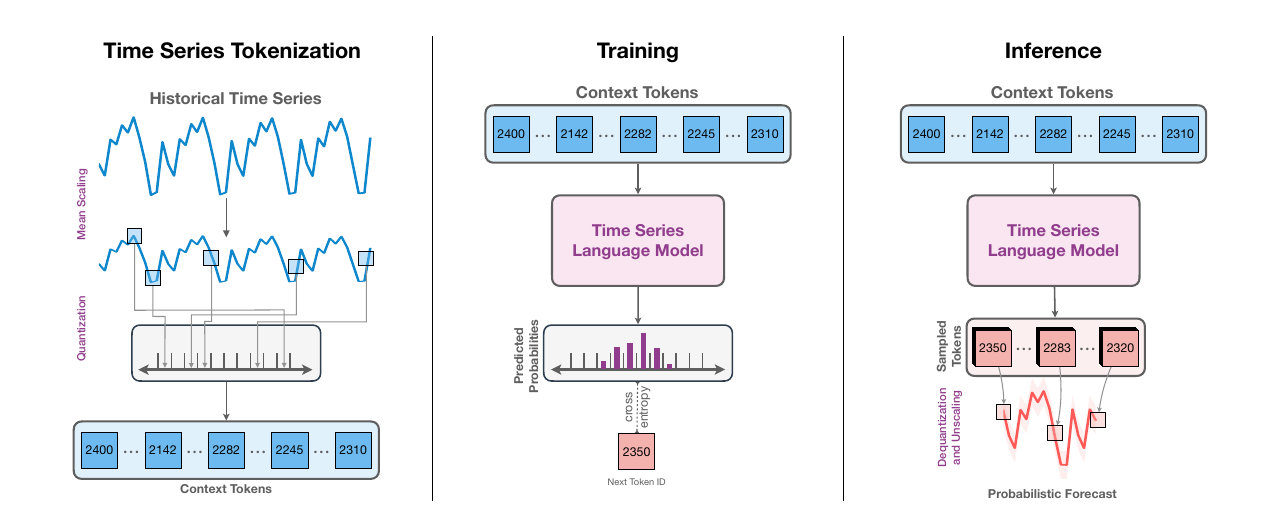
\includegraphics[width=\linewidth,height=3.20cm,keepaspectratio]{chronos-figure1.png}

      \vspace{0.13cm}
      \scriptsize\raggedright
      \begin{itemize}
        \setlength{\itemsep}{3pt}
        \item \textbf{Representation:} mean-scale the series, quantize values
          into bins, and map them to a fixed token vocabulary.
        \item \textbf{Architecture:} a T5 encoder--decoder learns next-token
          probabilities using cross-entropy.
        \item \textbf{Forecast:} autoregressive token samples are dequantized
          into trajectories. Inference is \textbf{stochastic}; the sampled
          trajectories define a \textbf{probabilistic forecast}.
      \end{itemize}
    \end{column}
    \begin{column}{0.30\linewidth}
      \tagbox{GoldLight}{\textbf{Chronos--T5 variants}}

      \vspace{0.18cm}
      \scriptsize
      \renewcommand{\arraystretch}{1.42}
      \setlength{\tabcolsep}{3pt}
      \begin{tabular}{L{1.20cm} C{1.05cm} C{1.22cm}}
        \toprule
        \textbf{Variant} & \textbf{Params} & \textbf{Enc./Dec.} \\
        \midrule
        Tiny  & 8M   & 4 / 4 \\
        Mini  & 20M  & 4 / 4 \\
        Small & 46M  & 6 / 6 \\
        Base  & 200M & 12 / 12 \\
        Large & 710M & 24 / 24 \\
        \bottomrule
      \end{tabular}

      \vspace{0.32cm}
      \small\raggedright
      The variants use the same tokenization and forecasting mechanism.
      Capacity increases through greater depth and width.
    \end{column}
  \end{columns}
\end{frame}

% -----------------------------------------------------------------------------
\begin{frame}{TimesFM: patch the signal, decode the future}
  \vspace{0.01cm}
  \begin{columns}[T,totalwidth=0.96\linewidth]
    \begin{column}{0.62\linewidth}
      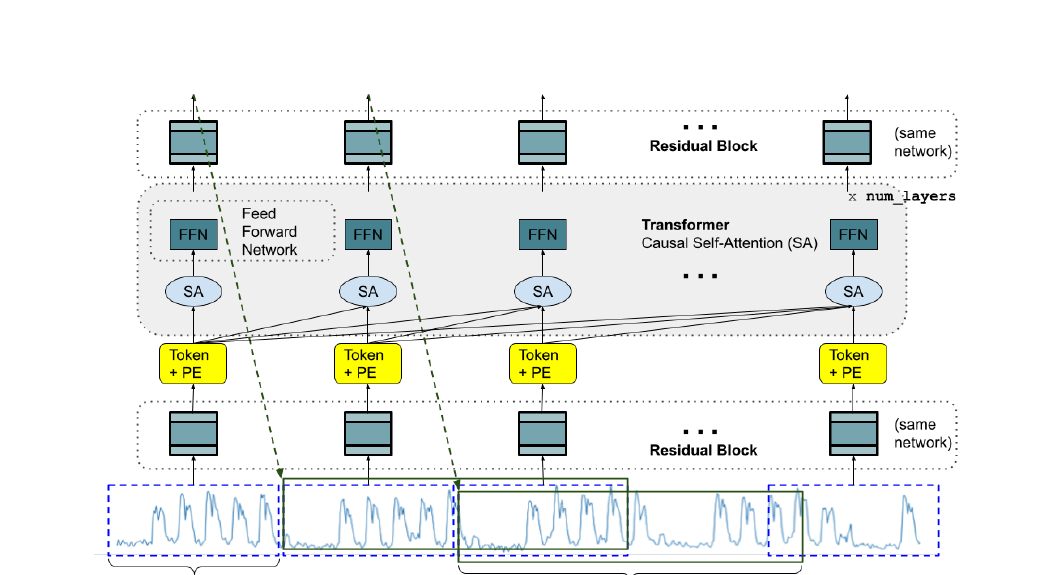
\includegraphics[width=\linewidth,height=5.40cm,keepaspectratio]{timesfm-figure1.png}
    \end{column}
    \begin{column}{0.32\linewidth}
      \tagbox{TealLight}{\textbf{Patch tokens}}
      \vspace{0.10cm}

      \scriptsize Non-overlapping blocks of 32 observations are normalized and
      projected into token embeddings.

      \vspace{0.19cm}
      \tagbox{PurpleLight}{\textbf{Decoder-only}}
      \vspace{0.10cm}

      \scriptsize Causal self-attention lets each patch representation use only
      its available history.

      \vspace{0.19cm}
      \tagbox{GoldLight}{\textbf{Multi-horizon}}
      \vspace{0.10cm}

      \scriptsize Each output head predicts a block of future time points;
      blocks are composed to reach the requested horizon.

      \vspace{0.25cm}
      \colorbox{GreenLight}{\parbox{0.92\linewidth}{\scriptsize
        \textbf{Forecast behavior}\par\vspace{2pt}
        TimesFM 2.5 directly outputs the mean and quantiles q10--q90.
        The values are \textbf{probabilistic forecasts}, but inference is
        \textbf{deterministic}: the same input returns the same distribution.}}
    \end{column}
  \end{columns}
\end{frame}

% -----------------------------------------------------------------------------
\begin{frame}{Moirai: one model for any frequency and variate count}
  \vspace{0.01cm}
  \begin{center}
    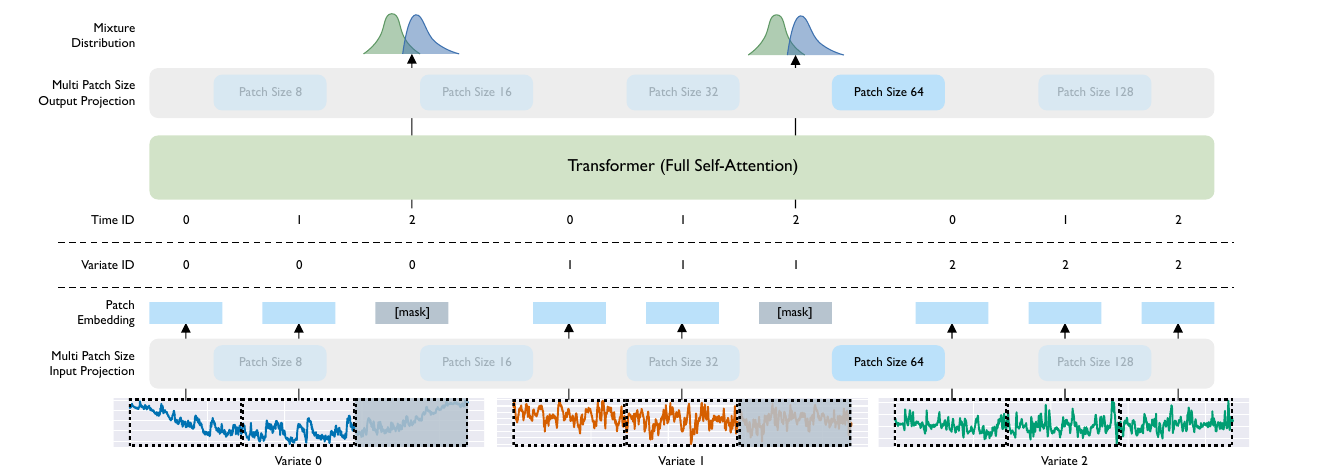
\includegraphics[width=0.95\linewidth,height=3.35cm,keepaspectratio]{moirai-figure2.png}
  \end{center}

  \vspace{0.16cm}
  \begin{columns}[T,totalwidth=0.94\linewidth]
    \begin{column}{0.29\linewidth}
      \tagbox{TealLight}{\textbf{Multiple patch sizes}}
      \vspace{0.09cm}

      \scriptsize A bank of input/output projections supports several patch
      lengths. The model can match its temporal resolution to series with
      different sampling frequencies and local dynamics.
    \end{column}
    \begin{column}{0.29\linewidth}
      \tagbox{PurpleLight}{\textbf{Any-variate attention}}
      \vspace{0.09cm}

      \scriptsize Patches from every variable are flattened into one token
      sequence. Time and variable identifiers preserve where each patch came
      from, so attention can learn both within- and cross-variable dependence.
    \end{column}
    \begin{column}{0.29\linewidth}
      \tagbox{GreenLight}{\textbf{Distribution forecast}}
      \vspace{0.09cm}

      \scriptsize Masked future patches are decoded into an uncertainty
      representation. The original Moirai uses a flexible mixture density;
      Moirai 2.0 directly predicts quantiles. Inference is deterministic.
    \end{column}
  \end{columns}
\end{frame}

% -----------------------------------------------------------------------------
\begin{frame}{Twelve datasets I: competition and archive panels}
  \vspace{0.14cm}
  \fontsize{8.3}{9.6}\selectfont
  \renewcommand{\arraystretch}{1.45}
  \setlength{\tabcolsep}{3.1pt}
  \begin{tabularx}{\linewidth}{L{2.15cm} L{2.45cm} C{1.75cm} Y}
    \toprule
    \textbf{Dataset} & \textbf{Domain} & \textbf{Series used} &
      \textbf{Main patterns} \\
    \midrule
    \rowcolor{TealLight}
    M1 Yearly & Business / economic & 20 &
      Trends and changes in level \\
    M3 Quarterly & Business / economic & 20 &
      Trends and quarterly cycles \\
    \rowcolor{TealLight}
    M4 Hourly & Mixed competition & 20 &
      Daily cycles and noise \\
    Weather (rain) & Environment & 20 &
      Many zeros and seasonal rain patterns \\
    \rowcolor{TealLight}
    Car Parts & Retail / inventory & 20 &
      Sparse demand with many zeros \\
    NN5 Weekly & Banking / ATM & 20 &
      Yearly patterns, holidays, changing demand \\
    \bottomrule
  \end{tabularx}
\end{frame}

% -----------------------------------------------------------------------------
\begin{frame}{Twelve datasets II: health, infrastructure, and macroeconomics}
  \vspace{0.14cm}
  \fontsize{8.15}{9.45}\selectfont
  \renewcommand{\arraystretch}{1.40}
  \setlength{\tabcolsep}{3.0pt}
  \begin{tabularx}{\linewidth}{L{2.25cm} L{2.55cm} C{1.75cm} Y}
    \toprule
    \textbf{Dataset} & \textbf{Domain} & \textbf{Series used} &
      \textbf{Main patterns} \\
    \midrule
    \rowcolor{GoldLight}
    National Illness & Public health & 1 &
      Yearly flu cycle and sudden peaks \\
    Traffic & Transport & 5 &
      Strong daily and weekly traffic cycles \\
    \rowcolor{GoldLight}
    PSM & Server telemetry & 5 &
      Sudden anomalies and noisy sensor data \\
    Elexon Demand & Energy & 1 &
      Weekly demand cycle and weather effects \\
    \rowcolor{GoldLight}
    USGS Streamflow & Hydrology & 5 &
      Yearly water cycle, floods, droughts, gaps \\
    BLS Macro & Macroeconomics & 3 &
      Long trends and structural changes \\
    \bottomrule
  \end{tabularx}
\end{frame}

% -----------------------------------------------------------------------------
\begin{frame}{Point and probabilistic forecast evaluation}
  \vspace{0.03cm}
  \begin{columns}[T,totalwidth=0.97\linewidth]
    \begin{column}{0.31\linewidth}
      \tagbox{TealLight}{\large\textbf{MASE} \; point}
      \vspace{0.14cm}

      \scriptsize
      \begin{center}
        \resizebox{0.98\linewidth}{!}{$\displaystyle
          \mathrm{MASE}=\frac{H^{-1}\sum_{h=1}^{H}|y_h-\hat y_h|}
          {(T-m)^{-1}\sum_{t=m+1}^{T}|y_t-y_{t-m}|}$}
      \end{center}
      Error scaled by an in-sample seasonal-naive error.
      It is comparable across units and datasets.

      \vspace{0.13cm}
      \good{$<1$} beats the scale; $=1$ matches it; \warn{$>1$} is worse.
    \end{column}
    \begin{column}{0.31\linewidth}
      \tagbox{GoldLight}{\large\textbf{WQL} \; quantiles}
      \vspace{0.14cm}

      \scriptsize
      \begin{center}
        \resizebox{0.98\linewidth}{!}{$\displaystyle
          \mathrm{WQL}=\frac{1}{|Q|}\sum_{q\in Q}
          \frac{2\sum_h\rho_q(y_h-\hat y_{q,h})}{\sum_h|y_h|}$}
      \end{center}
      Weighted quantile (pinball) loss on
      $Q=\{0.1,\ldots,0.9\}$, normalized by target magnitude.

      \vspace{0.13cm}
      Multiple quantiles reveal asymmetric risk and interval quality.
    \end{column}
    \begin{column}{0.31\linewidth}
      \tagbox{PurpleLight}{\large\textbf{CRPS} \; distribution}
      \vspace{0.14cm}

      \scriptsize
      \begin{center}
        \resizebox{0.98\linewidth}{!}{$\displaystyle
          \mathrm{CRPS}(F,y)=\int_{-\infty}^{\infty}
          \bigl(F(z)-\mathbf{1}\{y\le z\}\bigr)^2\,dz$}
      \end{center}
      Scores the entire predictive CDF against the observation;
      rewards \textbf{calibration} and \textbf{sharpness} jointly.

      \vspace{0.13cm}
      Implemented as a finite-quantile approximation from q10--q90.
    \end{column}
  \end{columns}

  \vspace{0.34cm}
  \begin{columns}[T,totalwidth=0.92\linewidth]
    \begin{column}{0.30\linewidth}
      \centering\scriptsize
      \colorbox{TealLight}{\parbox{0.90\linewidth}{\centering
        \textbf{Central forecast}\\How accurate is the median path?}}
    \end{column}
    \begin{column}{0.30\linewidth}
      \centering\scriptsize
      \colorbox{GoldLight}{\parbox{0.90\linewidth}{\centering
        \textbf{Quantile accuracy}\\Where are under- and over-predictions?}}
    \end{column}
    \begin{column}{0.30\linewidth}
      \centering\scriptsize
      \colorbox{PurpleLight}{\parbox{0.90\linewidth}{\centering
        \textbf{Distribution quality}\\How well does the predictive CDF match reality?}}
    \end{column}
  \end{columns}

  \vspace{0.22cm}
  \begin{center}\small\textbf{Together they separate scale-free point error from
  quantile and distributional quality; lower is better.}\end{center}
\end{frame}

\begin{frame}{Empirical winners across the three core losses}
  \vspace{0.04cm}
  \begin{center}
    \fontsize{8.4}{9.6}\selectfont
    \renewcommand{\arraystretch}{1.12}
    \setlength{\tabcolsep}{5.5pt}
    \begin{tabular}{L{3.05cm} C{3.20cm} C{3.20cm} C{3.20cm}}
      \toprule
      \textbf{Dataset} & \textbf{MASE} & \textbf{WQL} & \textbf{CRPS} \\
      \midrule
      M1 Yearly & \foundationwinner{TimesFM} & \classicalwinner{ARIMA} & \classicalwinner{ARIMA} \\
      M4 Hourly & \foundationwinner{Chronos Base} & \foundationwinner{Chronos Base} & \foundationwinner{Chronos Base} \\
      Weather & \foundationwinner{Chronos Base} & \foundationwinner{Moirai} & \foundationwinner{Moirai} \\
      M3 Quarterly & \foundationwinner{TimesFM} & \foundationwinner{TimesFM} & \foundationwinner{TimesFM} \\
      Car Parts & \foundationwinner{Moirai} & \foundationwinner{Moirai} & \foundationwinner{Moirai} \\
      NN5 Weekly & \foundationwinner{TimesFM} & \foundationwinner{TimesFM} & \foundationwinner{TimesFM} \\
      National Illness & \foundationwinner{TimesFM} & \foundationwinner{TimesFM} & \foundationwinner{TimesFM} \\
      Traffic & \foundationwinner{Moirai} & \foundationwinner{Moirai} & \foundationwinner{Moirai} \\
      PSM & \foundationwinner{Chronos Small} & \foundationwinner{Chronos Small} & \foundationwinner{Chronos Small} \\
      Elexon Demand & \foundationwinner{TimesFM} & \foundationwinner{TimesFM} & \foundationwinner{TimesFM} \\
      USGS Streamflow & \foundationwinner{Moirai} & \foundationwinner{TimesFM} & \foundationwinner{TimesFM} \\
      BLS Macro & \classicalwinner{Auto-ARIMA} & \foundationwinner{TimesFM} & \foundationwinner{TimesFM} \\
      \bottomrule
    \end{tabular}
  \end{center}

  \vspace{0.08cm}
  \begin{center}
    \scriptsize
    \tagbox{PurpleLight}{\textbf{foundation model}}
    \hspace{0.18cm}
    \tagbox{GoldLight}{\textbf{statistical model}}
    \hspace{0.28cm}
    Each cell is the lowest aggregate loss among 11 models; this is a
    \textbf{descriptive ranking}, not a significance claim.
  \end{center}
\end{frame}

% -----------------------------------------------------------------------------
\begin{frame}{How often each model records the lowest loss}
  \vspace{0.10cm}
  \begin{columns}[T,totalwidth=0.96\linewidth]
    \begin{column}{0.58\linewidth}
      \fontsize{8.2}{9.4}\selectfont
      \renewcommand{\arraystretch}{1.22}
      \setlength{\tabcolsep}{4.2pt}
      \begin{tabular}{L{3.15cm} C{0.82cm} C{0.82cm} C{0.82cm} C{0.82cm}}
        \toprule
        \textbf{Model} & \textbf{MASE} & \textbf{WQL} & \textbf{CRPS} & \textbf{Total} \\
        \midrule
        \rowcolor{GreenLight} TimesFM 2.5 200M & 5 & 6 & 6 & \textbf{17} \\
        Moirai 2.0 Small & 3 & 3 & 3 & \textbf{9} \\
        \rowcolor{Paper} Chronos Base & 2 & 1 & 1 & \textbf{4} \\
        Chronos Small & 1 & 1 & 1 & \textbf{3} \\
        \rowcolor{Paper} ARIMA(2,1,2) & 0 & 1 & 1 & \textbf{2} \\
        Auto-ARIMA & 1 & 0 & 0 & \textbf{1} \\
        \rowcolor{Paper} Chronos Mini & 0 & 0 & 0 & \textbf{0} \\
        Chronos Tiny & 0 & 0 & 0 & \textbf{0} \\
        \rowcolor{Paper} DeepAR & 0 & 0 & 0 & \textbf{0} \\
        Prophet & 0 & 0 & 0 & \textbf{0} \\
        \rowcolor{Paper} Seasonal Naive & 0 & 0 & 0 & \textbf{0} \\
        \midrule
        \textbf{Column total} & \textbf{12} & \textbf{12} & \textbf{12} & \textbf{36} \\
        \bottomrule
      \end{tabular}
    \end{column}

    \begin{column}{0.35\linewidth}
      \tagbox{GreenLight}{\large\textbf{36 comparisons}}
      \vspace{0.22cm}

      \small
      \begin{itemize}\setlength{\itemsep}{0.24cm}
        \item Each model is ranked on \textbf{MASE, WQL, and CRPS} across 12 datasets.
        \item A win means recording the lowest aggregate loss for one dataset
          under one metric.
        \item TimesFM records the lowest loss \textbf{17 times}; Moirai does so
          \textbf{9 times}.
        \item Across all comparisons, a foundation model ranks first
          \textbf{33 times}.
      \end{itemize}
    \end{column}
  \end{columns}
\end{frame}

% -----------------------------------------------------------------------------
\begin{frame}{When every foundation model beats every comparator}
  \vspace{0.02cm}
  \begin{center}
    \small
    \colorbox{TealLight}{\parbox{0.89\linewidth}{\centering
      \textbf{Strict family dominance:}\quad
      $\max_{m\in\mathrm{FM}}L(m)<\min_{m\in\mathrm{C}}L(m)$\quad---\quad
      even the weakest foundation model has lower aggregate loss than the
      strongest classical/conventional comparator.}}
  \end{center}

  \vspace{0.20cm}
  \begin{center}
    \fontsize{8.3}{9.6}\selectfont
    \renewcommand{\arraystretch}{1.22}
    \setlength{\tabcolsep}{5pt}
    \begin{tabular}{L{2.85cm} C{3.20cm} C{3.20cm} C{3.20cm}}
      \toprule
      \textbf{Dataset} & \textbf{MASE} & \textbf{WQL} & \textbf{CRPS} \\
      \midrule
      \rowcolor{GreenLight} M4 Hourly & $\checkmark$ Chronos Base & $\checkmark$ Chronos Base & $\checkmark$ Chronos Base \\
      PSM & $\checkmark$ Chronos Small & $\checkmark$ Chronos Small & $\checkmark$ Chronos Small \\
      \rowcolor{Paper} Elexon Demand & $\checkmark$ TimesFM & $\checkmark$ TimesFM & $\checkmark$ TimesFM \\
      USGS Streamflow & $\checkmark$ Moirai & $\checkmark$ TimesFM & $\checkmark$ TimesFM \\
      \rowcolor{Paper} Car Parts & \cellcolor{CoralLight}\textit{not strict} & $\checkmark$ Moirai & $\checkmark$ Moirai \\
      Traffic & \cellcolor{CoralLight}\textit{not strict} & $\checkmark$ Moirai & $\checkmark$ Moirai \\
      \bottomrule
    \end{tabular}
  \end{center}

  \vspace{0.18cm}
  \begin{center}
    \tagbox{GreenLight}{\textbf{16 strict comparisons}}
    \hspace{0.22cm}
    \small Four datasets satisfy the condition for all three losses; Car Parts
    and Traffic satisfy it for WQL and CRPS.
  \end{center}

\end{frame}

% -----------------------------------------------------------------------------
\begin{frame}{Clear empirical separation: M4 Hourly CRPS}
  \vspace{-0.02cm}
  \begin{center}
    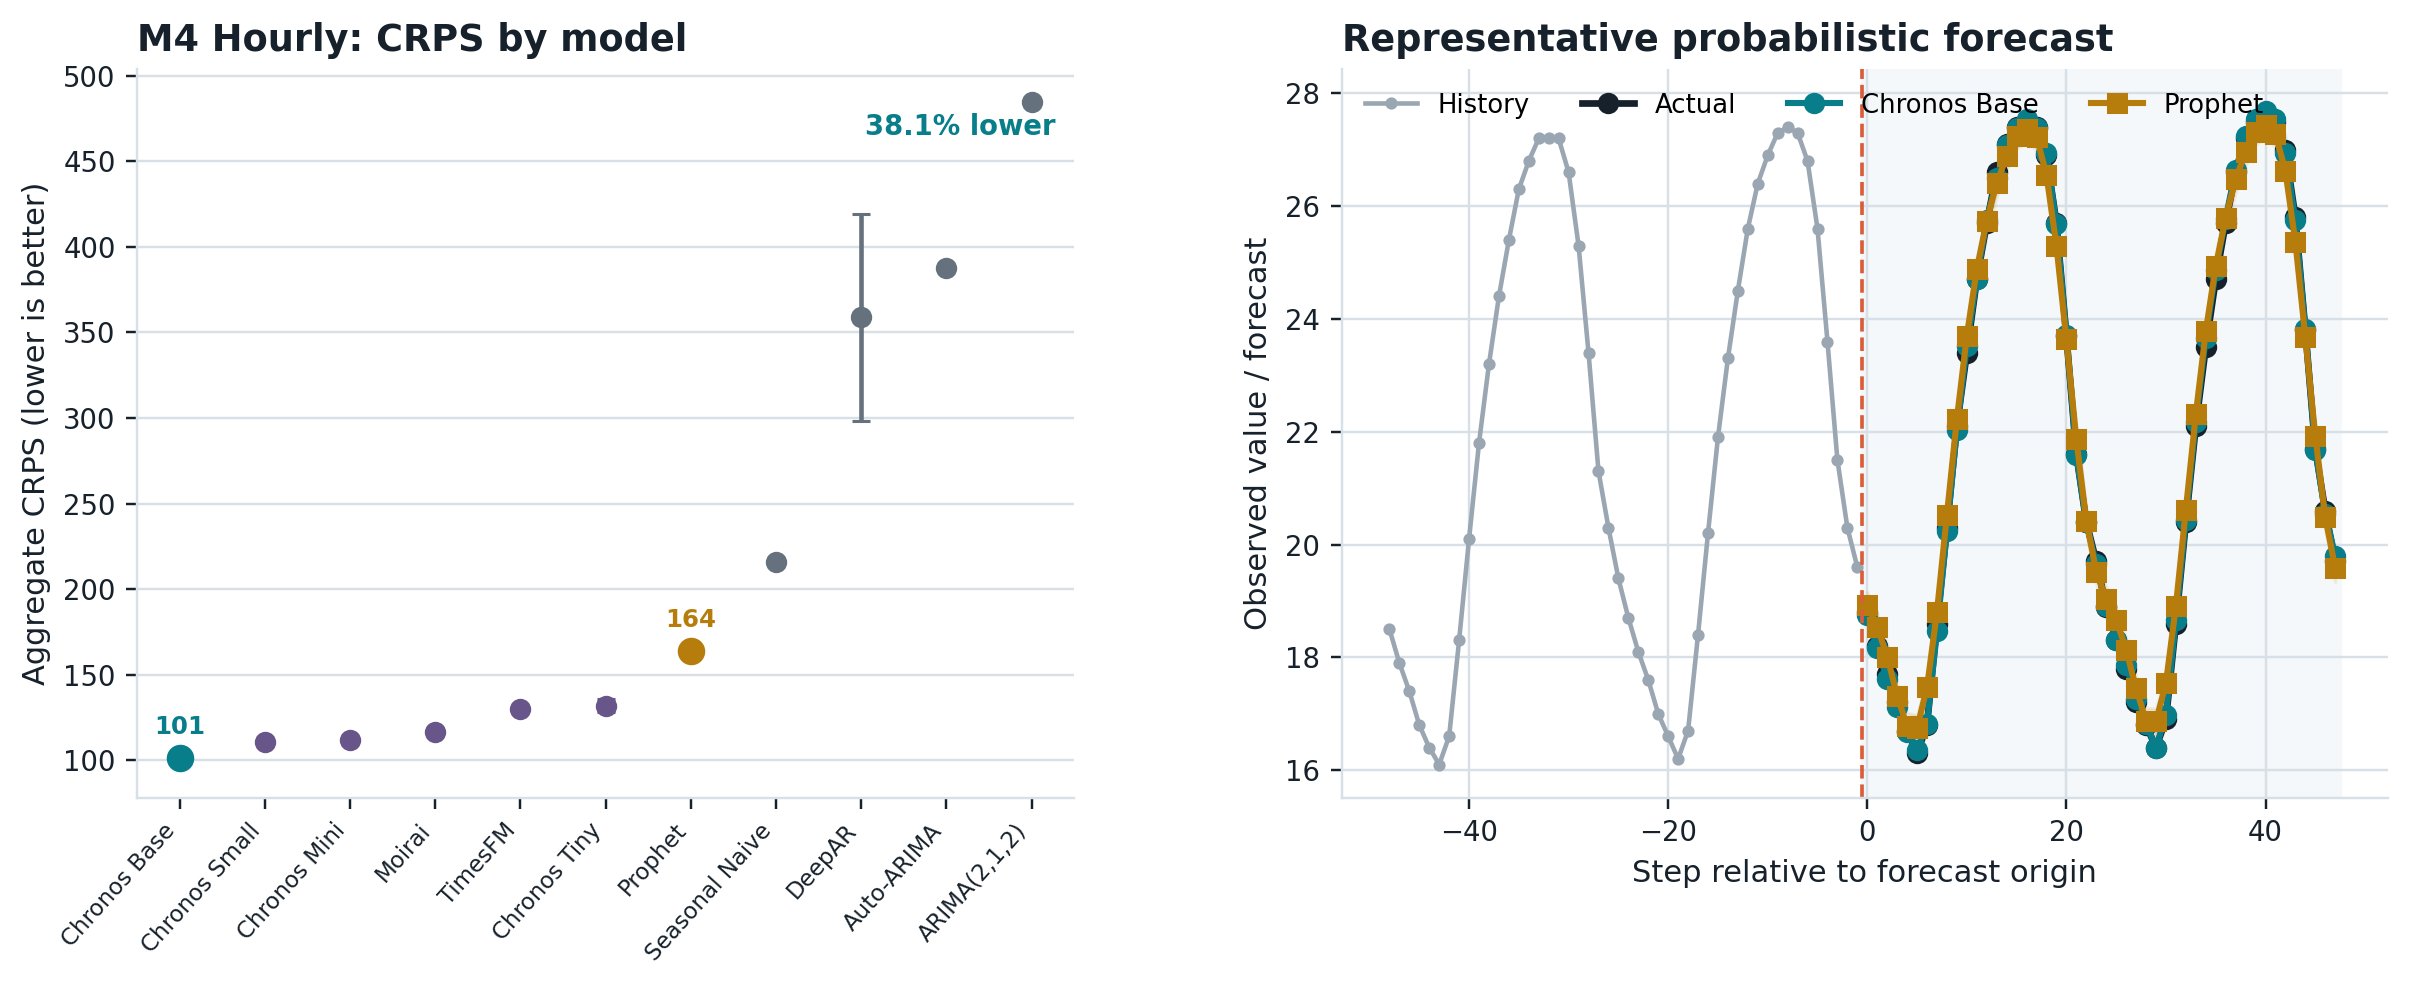
\includegraphics[width=0.94\linewidth]{m4-crps-separated-case.png}
  \end{center}

  \vspace{-0.04cm}
  \begin{center}\small
    \tagbox{TealLight}{\textbf{38.1\% lower aggregate CRPS}}
    \hspace{0.15cm}
    Similar point forecasts can still have differently scored distributions.
  \end{center}
\end{frame}

% -----------------------------------------------------------------------------
\begin{frame}{Clear empirical separation: PSM MASE}
  \vspace{-0.02cm}
  \begin{center}
    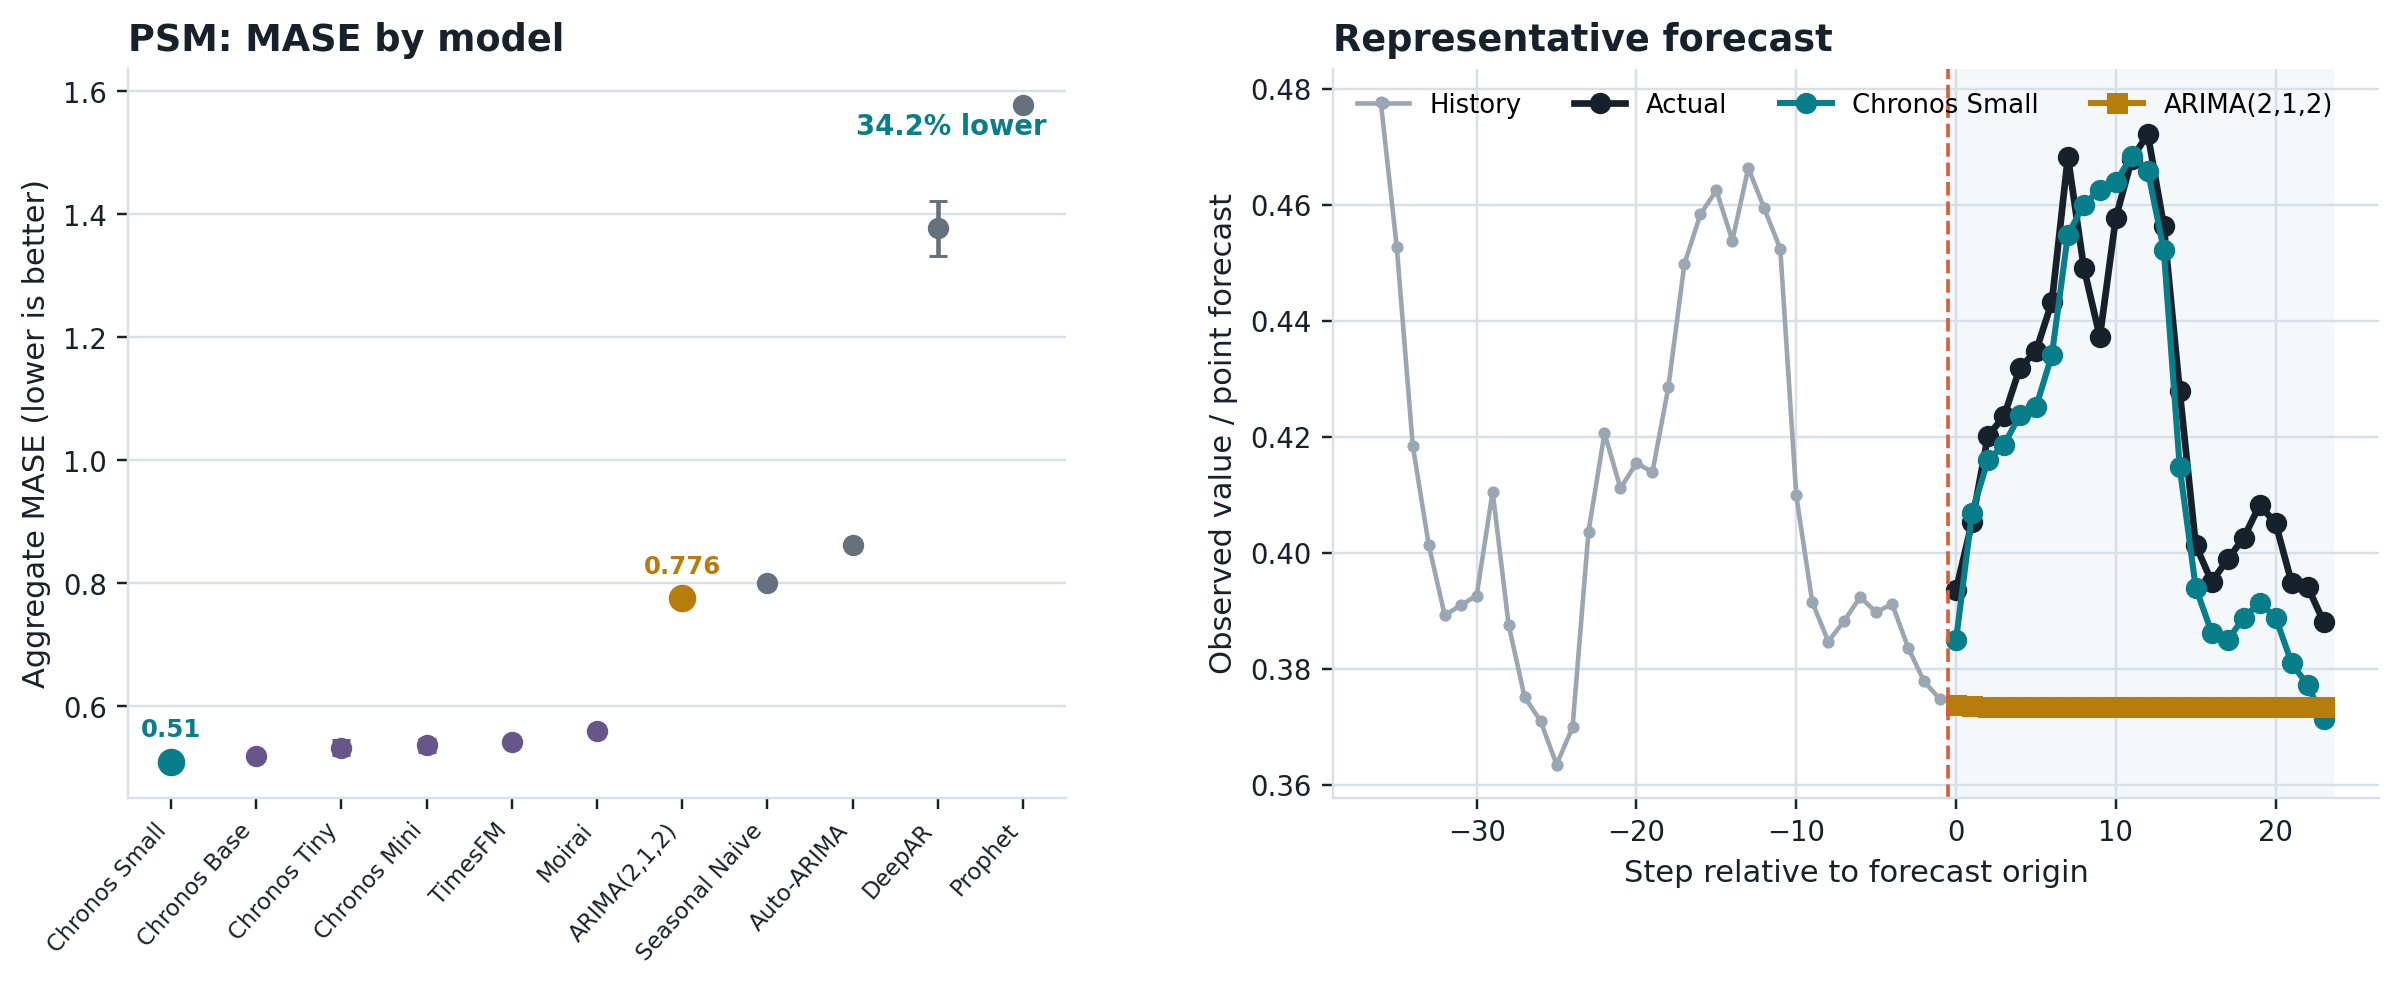
\includegraphics[width=0.94\linewidth]{psm-mase-separated-case.png}
  \end{center}

  \vspace{-0.04cm}
  \begin{center}\small
    \tagbox{TealLight}{\textbf{34.2\% lower aggregate MASE}}
    \hspace{0.15cm}
    Chronos Small follows the rise and decline; ARIMA remains nearly flat.
  \end{center}
\end{frame}

% -----------------------------------------------------------------------------
\begin{frame}{Where a foundation model ranks first in a mixed ordering}
  \vspace{0.02cm}
  \begin{center}
    \small
    \colorbox{PurpleLight}{\parbox{0.89\linewidth}{\centering
      \textbf{Mixed ordering:} a foundation model has the lowest loss, but at
      least one classical/conventional model still outranks another foundation
      model.}}
  \end{center}

  \vspace{0.16cm}
  \begin{center}
    \fontsize{7.7}{8.9}\selectfont
    \renewcommand{\arraystretch}{1.15}
    \setlength{\tabcolsep}{5pt}
    \begin{tabular}{L{2.85cm} C{3.20cm} C{3.20cm} C{3.20cm}}
      \toprule
      \textbf{Dataset} & \textbf{MASE} & \textbf{WQL} & \textbf{CRPS} \\
      \midrule
      Car Parts & \cellcolor{PurpleLight}\textbf{Moirai} & \cellcolor{TealLight}\textit{strict FM} & \cellcolor{TealLight}\textit{strict FM} \\
      \rowcolor{Paper} M1 Yearly & \cellcolor{PurpleLight}\textbf{TimesFM} & \cellcolor{GoldLight}\textit{classical first} & \cellcolor{GoldLight}\textit{classical first} \\
      M3 Quarterly & \cellcolor{PurpleLight}\textbf{TimesFM} & \cellcolor{PurpleLight}\textbf{TimesFM} & \cellcolor{PurpleLight}\textbf{TimesFM} \\
      \rowcolor{Paper} NN5 Weekly & \cellcolor{PurpleLight}\textbf{TimesFM} & \cellcolor{PurpleLight}\textbf{TimesFM} & \cellcolor{PurpleLight}\textbf{TimesFM} \\
      Weather & \cellcolor{PurpleLight}\textbf{Chronos Base} & \cellcolor{PurpleLight}\textbf{Moirai} & \cellcolor{PurpleLight}\textbf{Moirai} \\
      \rowcolor{Paper} National Illness & \cellcolor{PurpleLight}\textbf{TimesFM} & \cellcolor{PurpleLight}\textbf{TimesFM} & \cellcolor{PurpleLight}\textbf{TimesFM} \\
      Traffic & \cellcolor{PurpleLight}\textbf{Moirai} & \cellcolor{TealLight}\textit{strict FM} & \cellcolor{TealLight}\textit{strict FM} \\
      \rowcolor{Paper} BLS Macro & \cellcolor{GoldLight}\textit{classical first} & \cellcolor{PurpleLight}\textbf{TimesFM} & \cellcolor{PurpleLight}\textbf{TimesFM} \\
      \bottomrule
    \end{tabular}
  \end{center}

  \vspace{0.14cm}
  \begin{center}
    \tagbox{PurpleLight}{\textbf{17 mixed comparisons}}
    \hspace{0.14cm}
    \tagbox{TealLight}{\scriptsize strict FM dominance}
    \hspace{0.14cm}
    \tagbox{GoldLight}{\scriptsize classical model ranks first}
  \end{center}

  \vspace{0.08cm}
  \scriptsize\color{Muted}
  Purple cells name the empirical foundation-model leader.
\end{frame}

% -----------------------------------------------------------------------------
\begin{frame}{Close empirical contest: M1 Yearly MASE}
  \vspace{-0.02cm}
  \begin{center}
    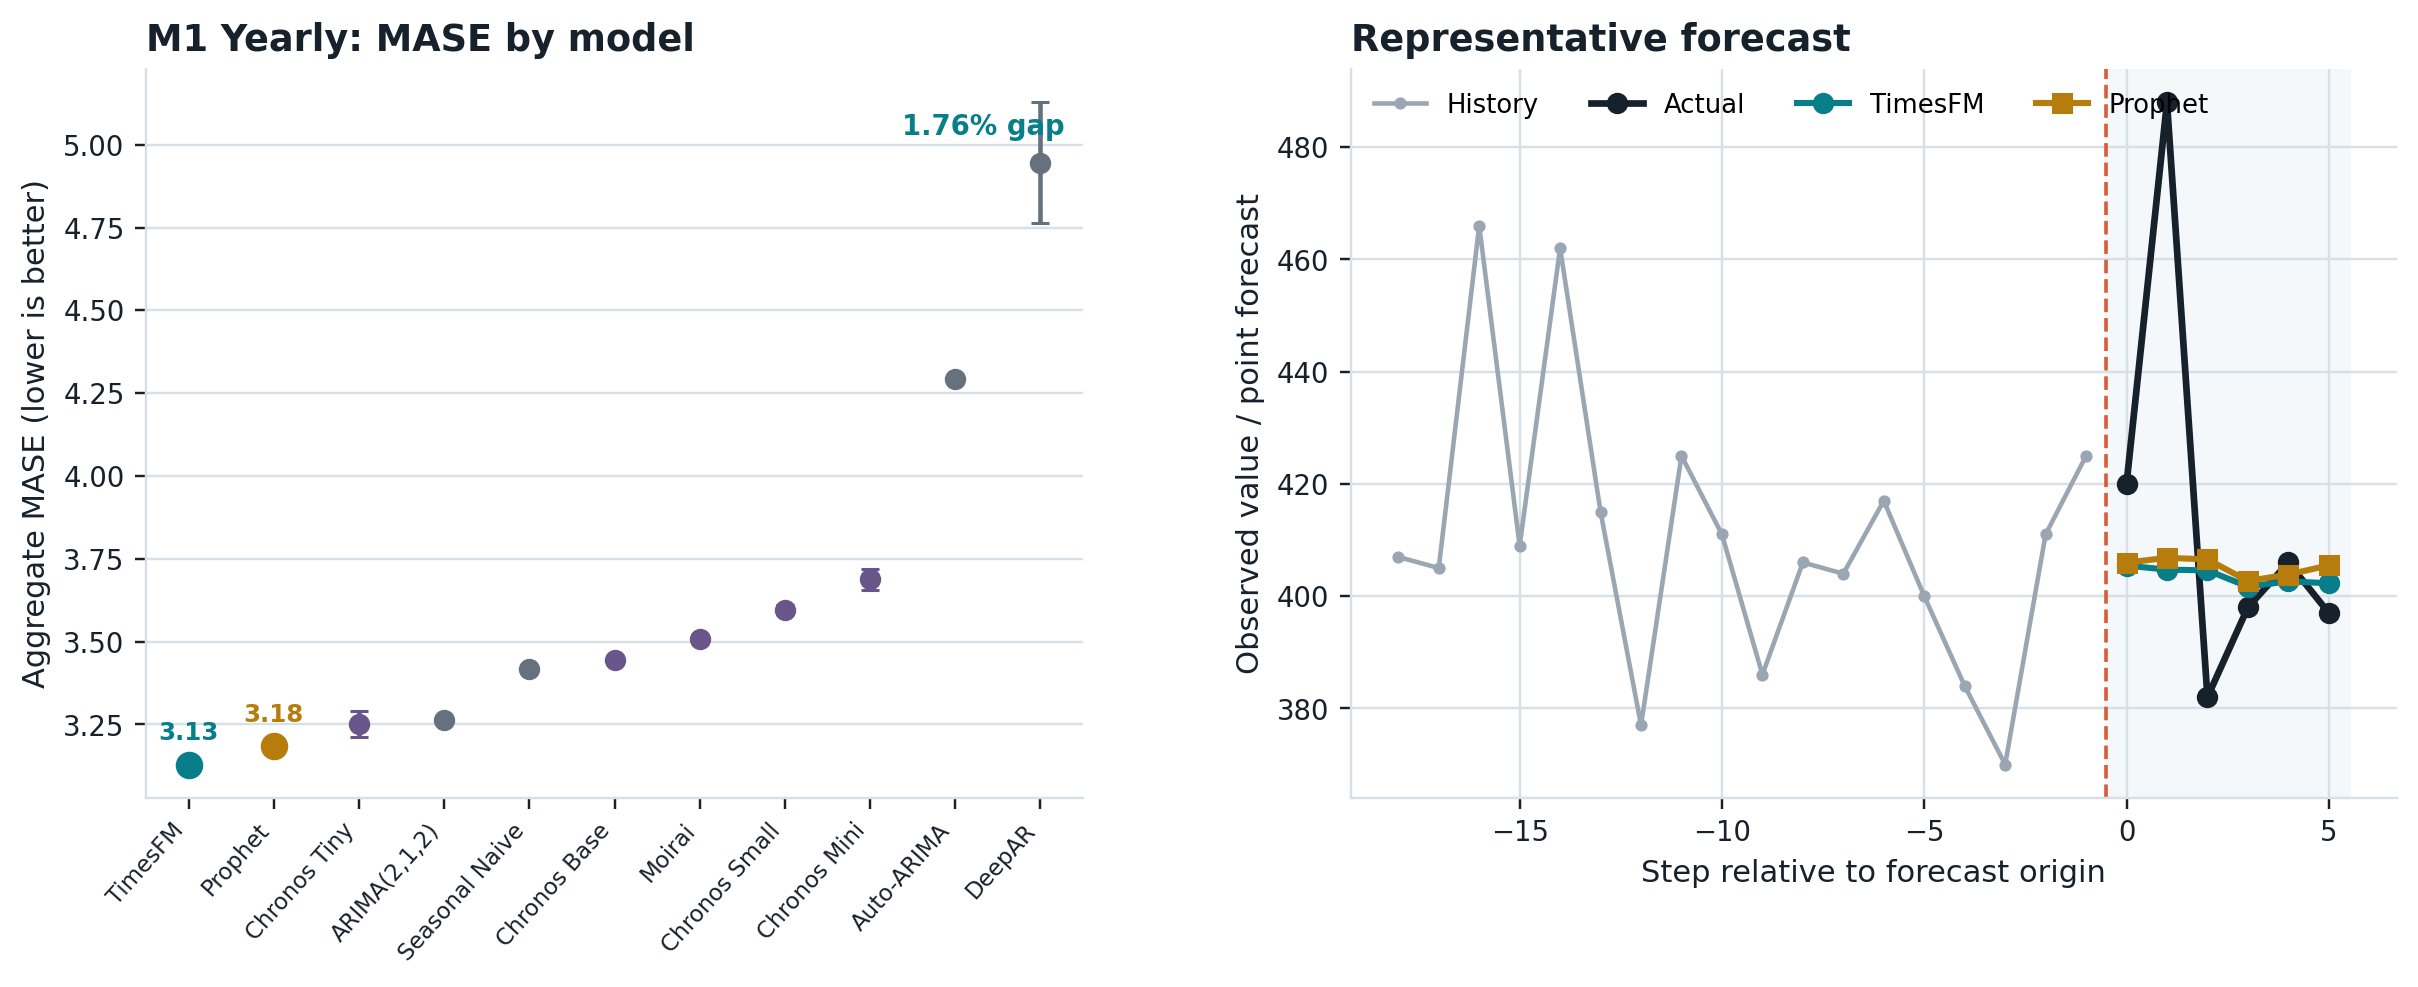
\includegraphics[width=0.94\linewidth]{m1-mase-close-case.png}
  \end{center}

  \vspace{-0.04cm}
  \begin{center}\small
    \tagbox{GoldLight}{\textbf{1.76\% aggregate gap}}
    \hspace{0.15cm}
    TimesFM ranks first, while Prophet is close and the forecasts nearly overlap.
  \end{center}
\end{frame}

% -----------------------------------------------------------------------------
\begin{frame}{Close empirical contest: M3 Quarterly WQL}
  \vspace{-0.02cm}
  \begin{center}
    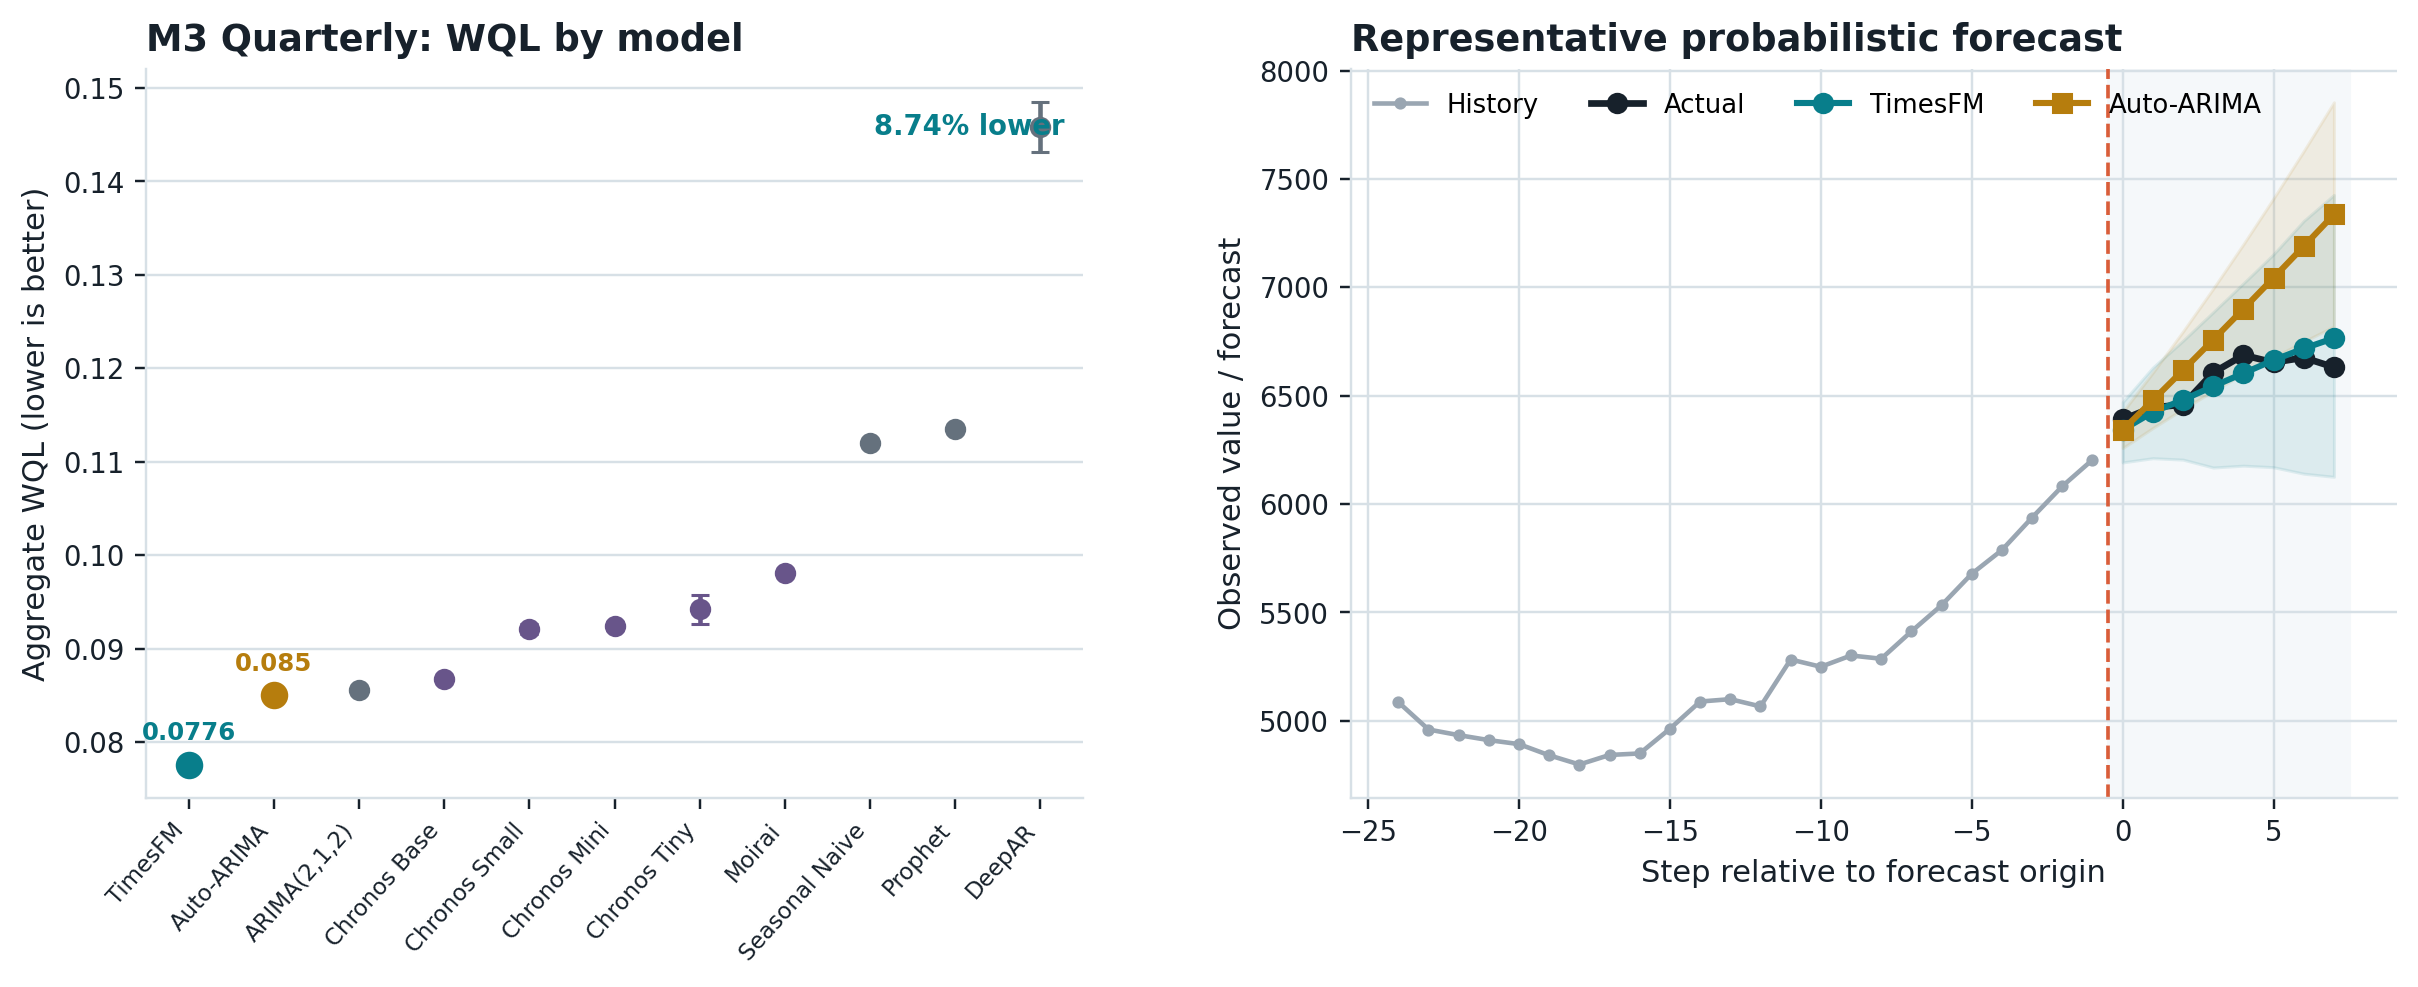
\includegraphics[width=0.94\linewidth]{m3-wql-close-case.png}
  \end{center}

  \vspace{-0.04cm}
  \begin{center}\small
    \tagbox{GoldLight}{\textbf{8.74\% lower aggregate WQL}}
    \hspace{0.15cm}
    TimesFM follows the realized level; Auto ARIMA drifts upward.
  \end{center}
\end{frame}

% -----------------------------------------------------------------------------
\begin{frame}{Where a classical model beats every foundation model}
  \vspace{0.06cm}
  \begin{center}
    \tagbox{GoldLight}{\large\textbf{3 of 36 cells}}
  \end{center}

  \vspace{0.22cm}
  \begin{center}
    \fontsize{8.4}{9.8}\selectfont
    \renewcommand{\arraystretch}{1.36}
    \setlength{\tabcolsep}{5pt}
    \begin{tabular}{L{2.45cm} C{1.25cm} L{3.10cm} L{3.10cm} C{1.65cm}}
      \toprule
      \textbf{Dataset} & \textbf{Loss} & \textbf{Classical winner} &
        \textbf{Best foundation model} & \textbf{Lower loss} \\
      \midrule
      M1 Yearly & WQL & ARIMA \; 0.0827 & Chronos Tiny \; 0.0944 & \textbf{12.4\%} \\
      \rowcolor{GoldLight} M1 Yearly & CRPS & ARIMA \; 202,882 & Chronos Tiny \; 231,712 & \textbf{12.4\%} \\
      BLS Macro & MASE & Auto-ARIMA \; 0.141 & TimesFM \; 0.174 & \textbf{18.8\%} \\
      \bottomrule
    \end{tabular}
  \end{center}

  \vspace{0.34cm}
  \begin{columns}[T,totalwidth=0.90\linewidth]
    \begin{column}{0.44\linewidth}
      \colorbox{GoldLight}{\parbox{0.91\linewidth}{\centering\small
        \textbf{M1 is the substantive exception}\par
        ARIMA leads both probabilistic losses across 60 paired tasks.}}
    \end{column}
    \begin{column}{0.44\linewidth}
      \colorbox{Paper}{\parbox{0.91\linewidth}{\centering\small
        \textbf{BLS remains tentative}\par
        Its MASE result is based on only seven paired tasks.}}
    \end{column}
  \end{columns}

  \vspace{0.16cm}
  \scriptsize\color{Muted}
  Values are aggregate losses; percentages compare the classical winner with
  the best-performing foundation model. Lower is better.
\end{frame}

% -----------------------------------------------------------------------------
\begin{frame}{Classical exception: M1 Yearly WQL}
  \vspace{-0.02cm}
  \begin{center}
    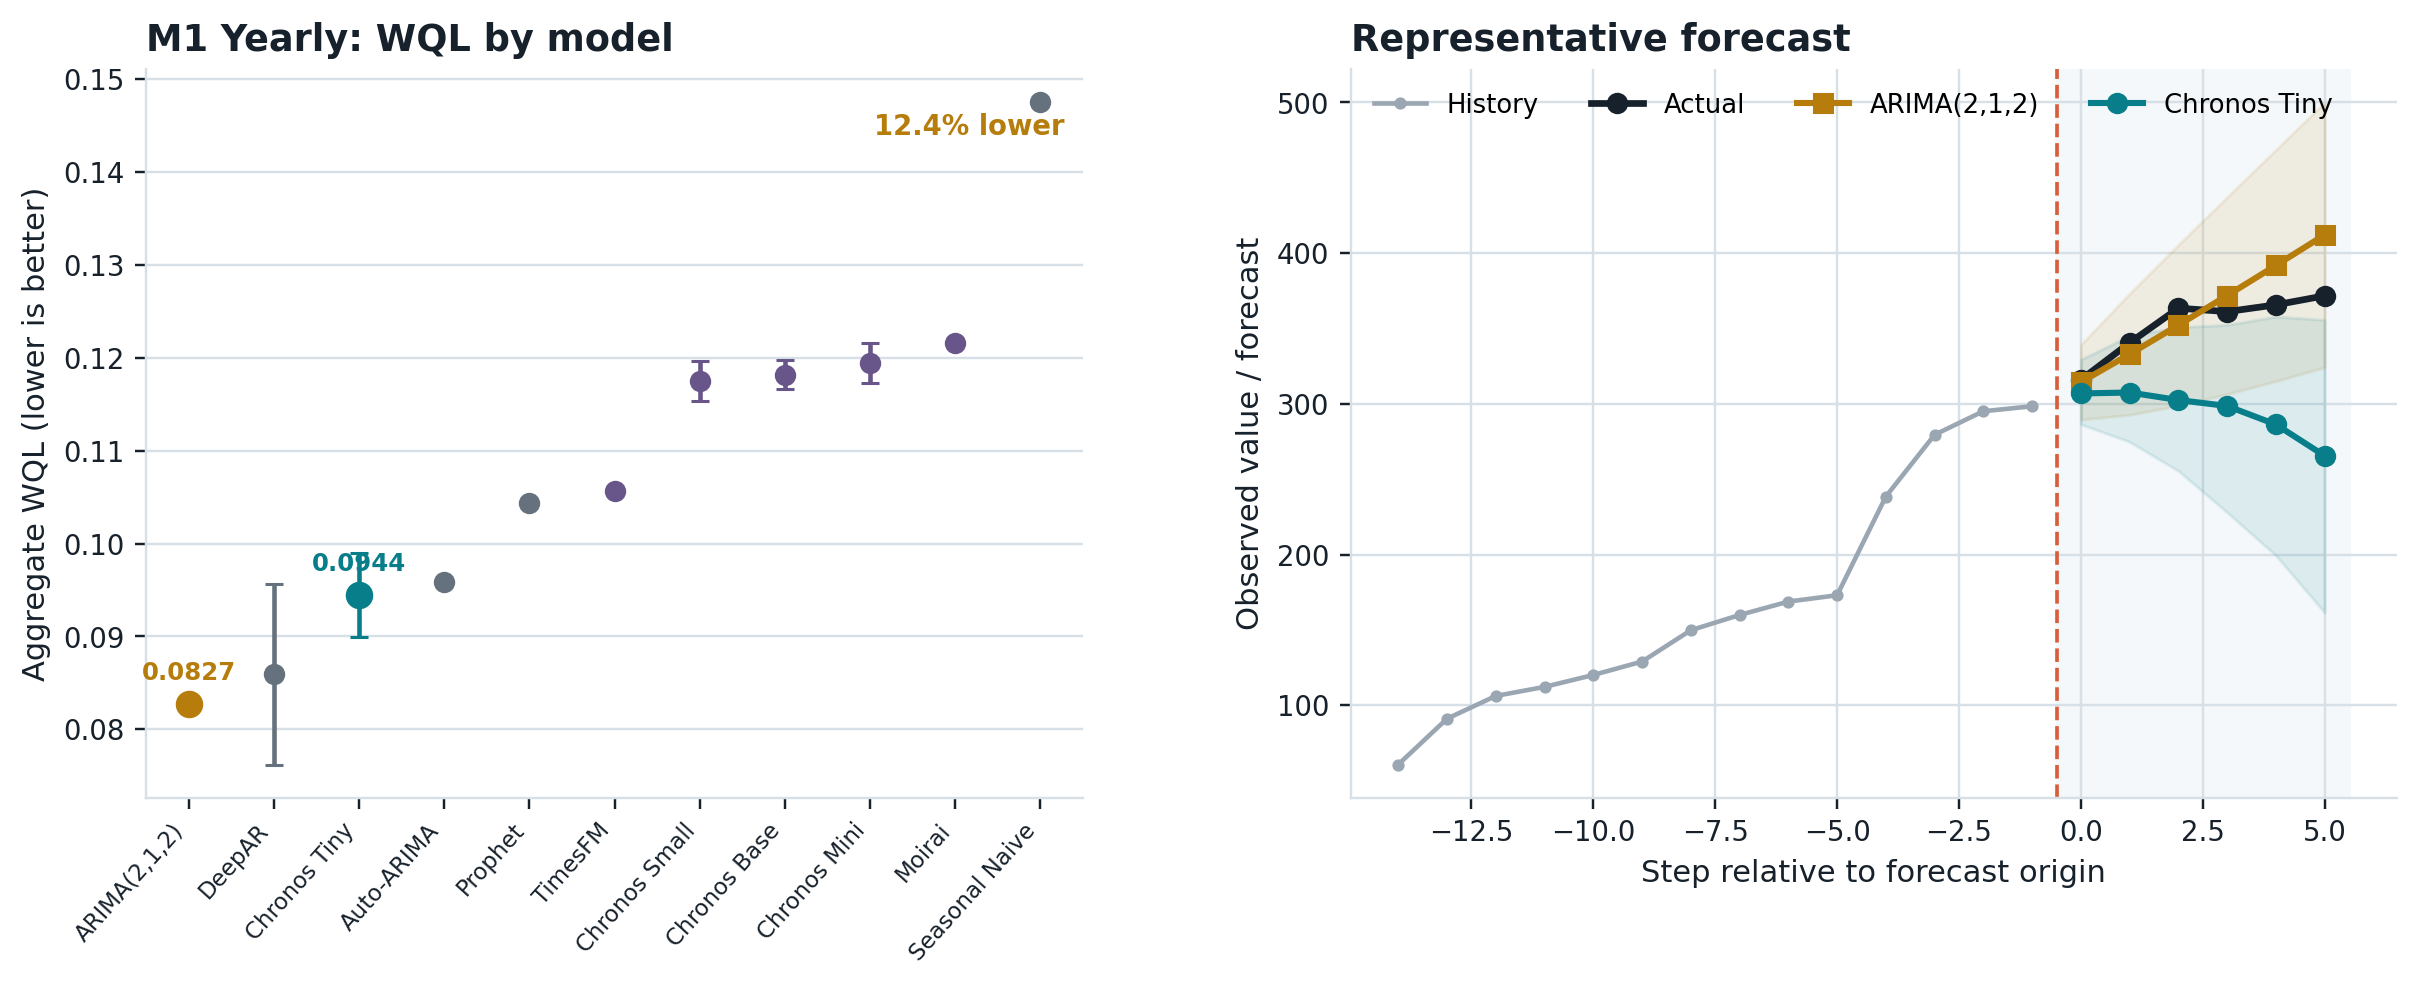
\includegraphics[width=0.94\linewidth]{m1-wql-classical-win.png}
  \end{center}

  \vspace{-0.04cm}
  \begin{center}\small
    \tagbox{GoldLight}{\textbf{12.4\% lower aggregate WQL}}
    \hspace{0.15cm}
    ARIMA follows the rise; its 10--90\% interval covers the observations.
  \end{center}
\end{frame}

% -----------------------------------------------------------------------------
\begin{frame}{Classical exception: BLS Macro MASE}
  \vspace{-0.02cm}
  \begin{center}
    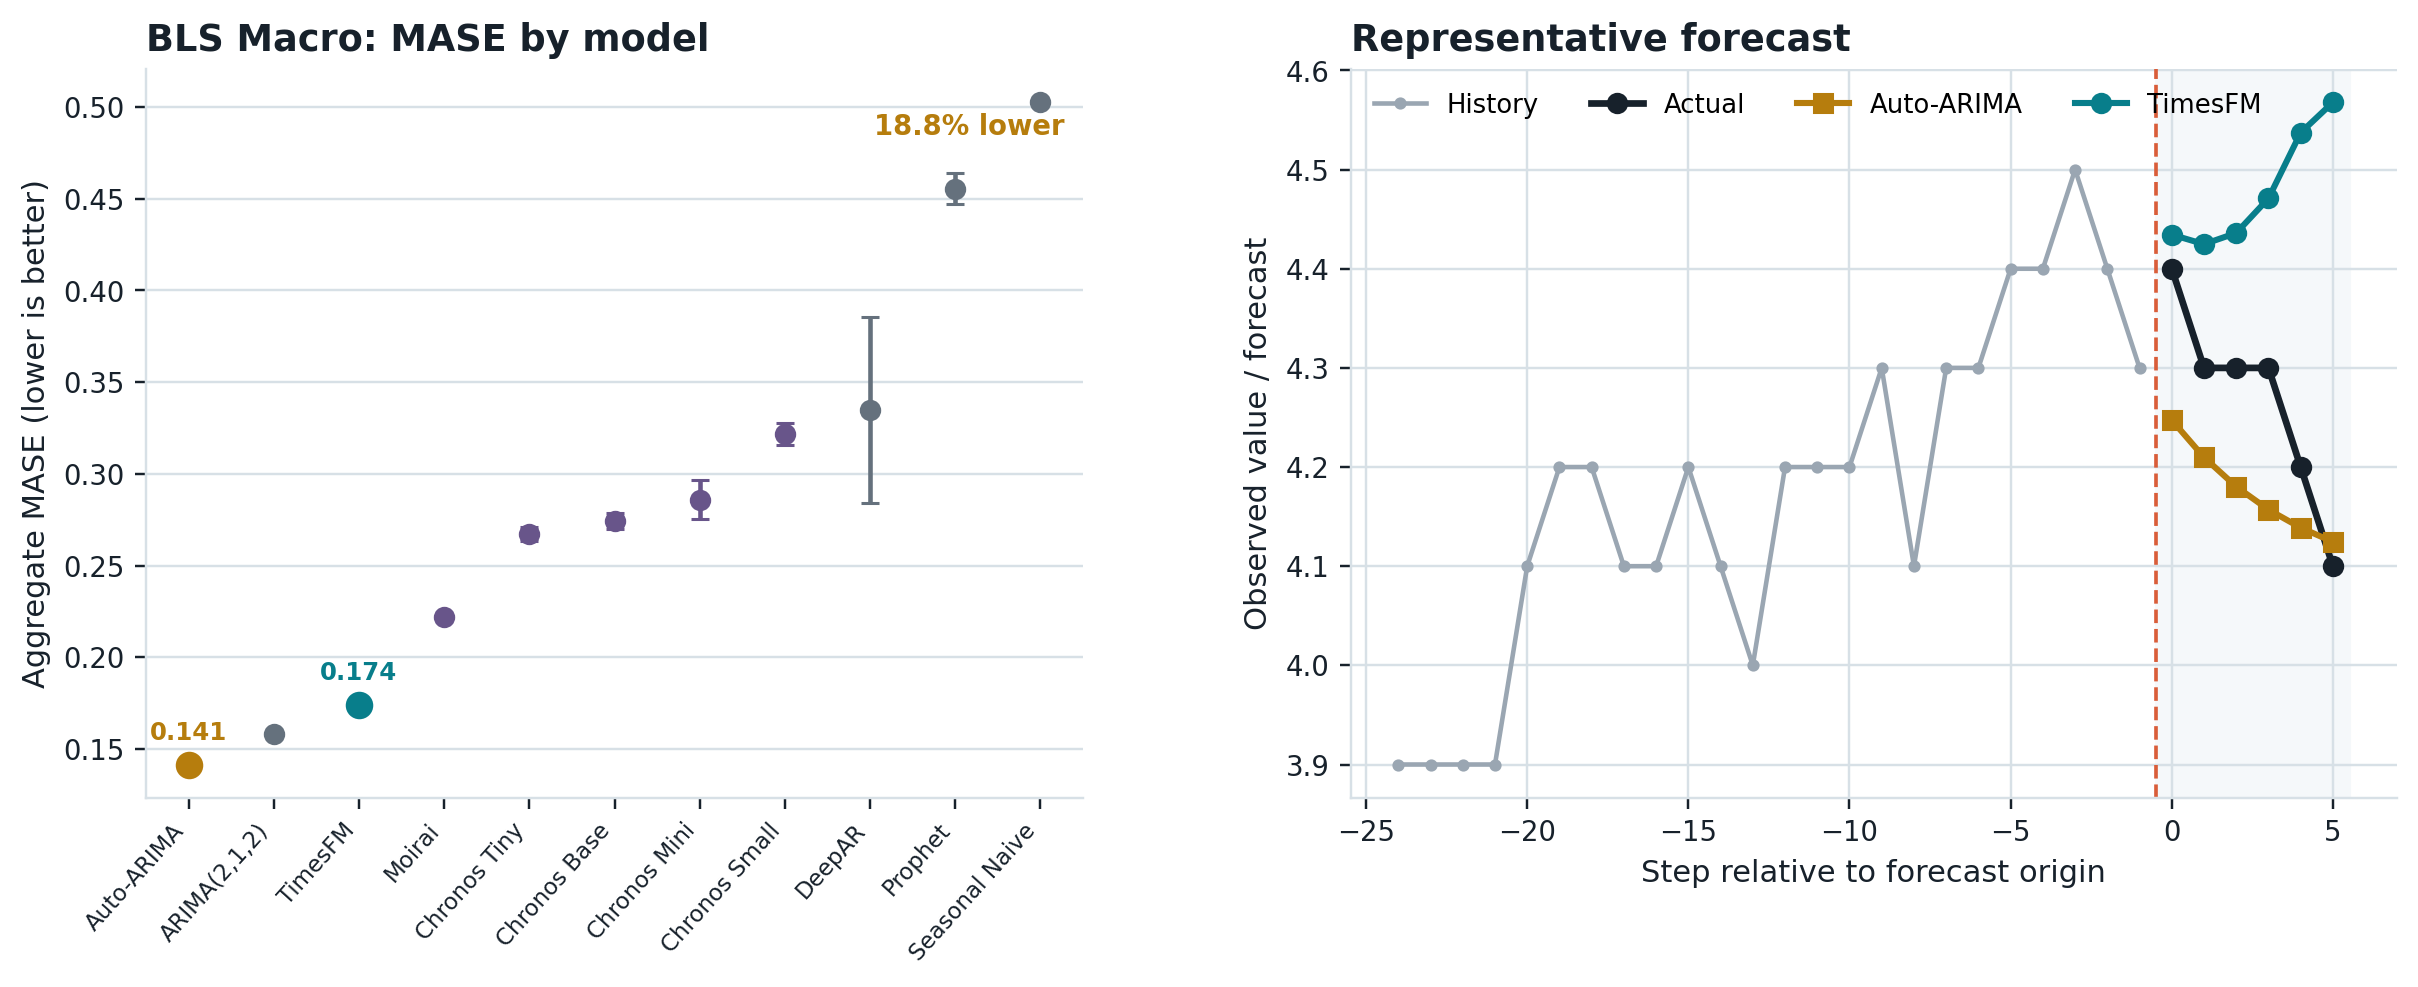
\includegraphics[width=0.94\linewidth]{bls-mase-classical-win.png}
  \end{center}

  \vspace{-0.04cm}
  \begin{center}\small
    \tagbox{GoldLight}{\textbf{18.8\% lower aggregate MASE}}
    \hspace{0.15cm}
    Auto-ARIMA follows the decline; TimesFM extrapolates upward.
  \end{center}
\end{frame}

% -----------------------------------------------------------------------------
\begin{frame}{How to interpret the repetition test}
  \vspace{0.02cm}
  \begin{center}
    \colorbox{Paper}{\parbox{0.91\linewidth}{\centering
      \small\bfseries Why are 22 \(p\)-values adjusted?\par
      \vspace{0.07cm}
      \begin{tabular}{C{3.15cm} c C{3.15cm} c C{3.15cm}}
        \shortstack{\color{Teal}\fontsize{17}{18}\selectfont\bfseries 36\\[-1pt]
          \color{Ink}\fontsize{7.2}{8.0}\selectfont comparisons\\
          \color{Muted}\fontsize{6.4}{7.1}\selectfont 12 datasets \(\times\) 3 losses}
        & \(\boldsymbol{-}\) &
        \shortstack{\color{Purple}\fontsize{17}{18}\selectfont\bfseries 14\\[-1pt]
          \color{Ink}\fontsize{7.2}{8.0}\selectfont SI cases\\
          \color{Muted}\fontsize{6.4}{7.1}\selectfont no numerical \(p\)-value}
        & \(\boldsymbol{=}\) &
        \shortstack{\color{Teal}\fontsize{17}{18}\selectfont\bfseries 22\\[-1pt]
          \color{Ink}\fontsize{7.2}{8.0}\selectfont numerical \(p\)-values\\
          \color{Muted}\fontsize{6.4}{7.1}\selectfont adjusted together}
      \end{tabular}}}
  \end{center}

  \vspace{0.11cm}
  \begin{center}\fontsize{8.5}{9.8}\selectfont
    Holm correction treats the 22 values as one family, limiting false positives
    caused by testing many comparisons.
  \end{center}

  \vspace{0.14cm}
  \begin{center}
    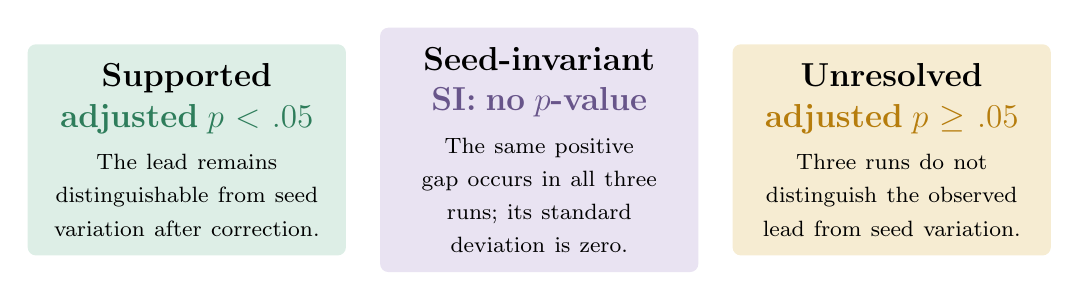
\begin{tikzpicture}[
      resultcard/.style={
        rounded corners=3pt,
        text width=3.55cm,
        minimum height=2.45cm,
        inner sep=7pt,
        align=center
      }
    ]
      \node[resultcard,fill=GreenLight] (supported) {
        {\large\bfseries Supported}\par
        \vspace{0.09cm}
        {\color{Green}\fontsize{12.5}{15}\selectfont\bfseries adjusted \(p<.05\)}\par
        \vspace{0.12cm}
        {\fontsize{8.1}{9.4}\selectfont
          The lead remains distinguishable from seed variation after correction.}
      };
      \node[resultcard,fill=PurpleLight,right=0.42cm of supported] (invariant) {
        {\large\bfseries Seed-invariant}\par
        \vspace{0.09cm}
        {\color{Purple}\fontsize{12.5}{15}\selectfont\bfseries SI: no \(p\)-value}\par
        \vspace{0.12cm}
        {\fontsize{8.1}{9.4}\selectfont
          The same positive gap occurs in all three runs; its standard deviation is zero.}
      };
      \node[resultcard,fill=GoldLight,right=0.42cm of invariant] (unresolved) {
        {\large\bfseries Unresolved}\par
        \vspace{0.09cm}
        {\color{Gold}\fontsize{12.5}{15}\selectfont\bfseries adjusted \(p\geq.05\)}\par
        \vspace{0.12cm}
        {\fontsize{8.1}{9.4}\selectfont
          Three runs do not distinguish the observed lead from seed variation.}
      };
    \end{tikzpicture}
  \end{center}

  \vspace{0.20cm}
  \begin{center}
    \colorbox{TealLight}{\parbox{0.76\linewidth}{\centering\fontsize{7.8}{9.0}\selectfont
      \textbf{Scope:} repeatability across three random seeds.}}
  \end{center}
\end{frame}

% -----------------------------------------------------------------------------
\begin{frame}{Do the rankings persist across random seeds?}
  \vspace{-0.02cm}
  \begin{center}
    \colorbox{Paper}{\parbox{0.91\linewidth}{\centering\fontsize{6.7}{7.4}\selectfont
      Winner versus the best model from the opposite family:\quad
      $d_r=L_{\mathrm{opposite},r}-L_{\mathrm{winner},r}$,\quad
      $H_0:\mathbb{E}[d]\leq0$,\quad one-sided paired $t$ test, $n=3$.}}
  \end{center}

  \vspace{0.04cm}
  \begin{center}
    \fontsize{7.2}{8.0}\selectfont
    \renewcommand{\arraystretch}{1.02}
    \setlength{\tabcolsep}{6.5pt}
    \begin{tabular}{L{3.65cm} C{2.40cm} C{2.40cm} C{2.40cm}}
      \toprule
      \textbf{Dataset} & \textbf{MASE} & \textbf{WQL} & \textbf{CRPS} \\
      \midrule
      Car Parts & \cellcolor{GreenLight}\textbf{0.025} & \cellcolor{PurpleLight}\textbf{SI} & \cellcolor{PurpleLight}\textbf{SI} \\
      \rowcolor{Paper} M1 Yearly & \cellcolor{GreenLight}\textbf{0.004} & \cellcolor{GoldLight}0.068 & \cellcolor{GoldLight}0.068 \\
      M3 Quarterly & \cellcolor{PurpleLight}\textbf{SI} & \cellcolor{PurpleLight}\textbf{SI} & \cellcolor{PurpleLight}\textbf{SI} \\
      \rowcolor{Paper} M4 Hourly & \cellcolor{GreenLight}\textbf{$<0.001$} & \cellcolor{GreenLight}\textbf{0.010} & \cellcolor{GreenLight}\textbf{0.010} \\
      NN5 Weekly & \cellcolor{GreenLight}\textbf{0.047} & \cellcolor{GreenLight}\textbf{0.025} & \cellcolor{GreenLight}\textbf{0.025} \\
      \rowcolor{Paper} Weather & \cellcolor{GoldLight}0.091 & \cellcolor{GreenLight}\textbf{0.025} & \cellcolor{GreenLight}\textbf{0.025} \\
      National Illness & \cellcolor{GreenLight}\textbf{$<0.001$} & \cellcolor{GreenLight}\textbf{$<0.001$} & \cellcolor{GreenLight}\textbf{$<0.001$} \\
      \rowcolor{Paper} PSM & \cellcolor{GreenLight}\textbf{$<0.001$} & \cellcolor{GreenLight}\textbf{$<0.001$} & \cellcolor{GreenLight}\textbf{$<0.001$} \\
      Traffic & \cellcolor{PurpleLight}\textbf{SI} & \cellcolor{PurpleLight}\textbf{SI} & \cellcolor{PurpleLight}\textbf{SI} \\
      \rowcolor{Paper} BLS Macro & \cellcolor{PurpleLight}\textbf{SI} & \cellcolor{PurpleLight}\textbf{SI} & \cellcolor{PurpleLight}\textbf{SI} \\
      Elexon Demand & \cellcolor{PurpleLight}\textbf{SI} & \cellcolor{PurpleLight}\textbf{SI} & \cellcolor{GreenLight}\textbf{$<0.001$} \\
      \rowcolor{Paper} USGS Streamflow & \cellcolor{PurpleLight}\textbf{SI} & \cellcolor{GoldLight}0.052 & \cellcolor{GoldLight}0.052 \\
      \bottomrule
    \end{tabular}
  \end{center}

  \vspace{0.04cm}
  \begin{center}
    \tagbox{GreenLight}{\scriptsize\textbf{17 significant}}
    \hspace{0.12cm}
    \tagbox{PurpleLight}{\scriptsize\textbf{14 seed invariant}}
    \hspace{0.12cm}
    \tagbox{GoldLight}{\scriptsize\textbf{5 unresolved}}
  \end{center}

  \vspace{0.02cm}
  \fontsize{6.2}{7.0}\selectfont\color{Muted}
  Holm-adjusted $p$ values cover the 22 finite tests. SI means the same positive
  gap occurred in all three runs, so finite $t$ and $p$ values do not exist.
  The table measures repeatability across the three random seeds only.
\end{frame}

\begin{frame}[t]{95\% Model Confidence Set: method and results}
  \begin{center}
    \tagbox{Paper}{\scriptsize\textbf{11 candidate models}}
    \quad\(\longrightarrow\)\quad
    \tagbox{TealLight}{\scriptsize\textbf{test equality, remove the weakest, repeat}}
    \quad\(\longrightarrow\)\quad
    \tagbox{PurpleLight}{\scriptsize\textbf{95\% MCS}}
  \end{center}

  \vspace{0cm}
  \begin{center}\fontsize{6.5}{7.2}\selectfont
    MCS starts with all 11 models, tests equal predictive ability on paired
    losses, and removes the weakest after a rejection. The final 95\% set
    contains models not distinguished from the best.
    Each cell is \textbf{MCS size / opposite-family flag}: 1 means the best
    opposite-family model is excluded; 0 means it remains.
  \end{center}

  \vspace{0cm}
  \begin{center}
    \fontsize{7.2}{7.8}\selectfont
    \renewcommand{\arraystretch}{0.85}
    \setlength{\tabcolsep}{6.2pt}
    \begin{tabular}{L{3.45cm} C{2.58cm} C{2.58cm} C{2.58cm}}
      \toprule
      \textbf{Dataset} & \textbf{MASE} & \textbf{WQL} & \textbf{CRPS} \\
      \midrule
      M1 Yearly & \cellcolor{CoralLight}\textbf{9/0} & \cellcolor{CoralLight}\textbf{11/0} & \cellcolor{CoralLight}\textbf{11/0} \\
      \rowcolor{Paper} M4 Hourly & \cellcolor{GoldLight}\textbf{6/1} & \cellcolor{CoralLight}\textbf{11/0} & \cellcolor{CoralLight}\textbf{11/0} \\
      Weather & \cellcolor{CoralLight}\textbf{8/0} & \cellcolor{PurpleLight}\textbf{2/1} & \cellcolor{GreenLight}\textbf{1/1} \\
      \rowcolor{Paper} M3 Quarterly & \cellcolor{GoldLight}\textbf{4/0} & \cellcolor{PurpleLight}\textbf{2/1} & \cellcolor{GoldLight}\textbf{5/0} \\
      Car Parts & \cellcolor{GoldLight}\textbf{7/0} & \cellcolor{GoldLight}\textbf{7/1} & \cellcolor{GoldLight}\textbf{7/1} \\
      \rowcolor{Paper} NN5 Weekly & \cellcolor{GreenLight}\textbf{1/1} & \cellcolor{GreenLight}\textbf{1/1} & \cellcolor{GreenLight}\textbf{1/1} \\
      National Illness & \cellcolor{GoldLight}\textbf{7/0} & \cellcolor{GoldLight}\textbf{5/1} & \cellcolor{GoldLight}\textbf{5/1} \\
      \rowcolor{Paper} Traffic & \cellcolor{GoldLight}\textbf{6/0} & \cellcolor{GoldLight}\textbf{5/1} & \cellcolor{GoldLight}\textbf{5/1} \\
      PSM & \cellcolor{GoldLight}\textbf{7/1} & \cellcolor{GoldLight}\textbf{7/1} & \cellcolor{GoldLight}\textbf{7/1} \\
      \rowcolor{Paper} Elexon Demand & \cellcolor{PurpleLight}\textbf{3/1} & \cellcolor{PurpleLight}\textbf{2/1} & \cellcolor{PurpleLight}\textbf{2/1} \\
      USGS Streamflow & \cellcolor{CoralLight}\textbf{8/0} & \cellcolor{CoralLight}\textbf{11/0} & \cellcolor{CoralLight}\textbf{11/0} \\
      \rowcolor{Paper} BLS Macro & \cellcolor{GoldLight}\textbf{5/0} & \cellcolor{CoralLight}\textbf{11/0} & \cellcolor{CoralLight}\textbf{11/0} \\
      \bottomrule
    \end{tabular}
  \end{center}

  \vspace{-0.17cm}
  \begin{center}
    \tagbox{GreenLight}{\fontsize{6.4}{7.1}\selectfont\textbf{1: unique}}
    \hspace{0.08cm}
    \tagbox{PurpleLight}{\fontsize{6.4}{7.1}\selectfont\textbf{2--3: narrow}}
    \hspace{0.08cm}
    \tagbox{GoldLight}{\fontsize{6.4}{7.1}\selectfont\textbf{4--7: competitive}}
    \hspace{0.08cm}
    \tagbox{CoralLight}{\fontsize{6.4}{7.1}\selectfont\textbf{8--11: broad}}
  \end{center}
\end{frame}

% -----------------------------------------------------------------------------
\begin{frame}{NN5 Weekly: CRPS leaves one model in the MCS}
  \vspace{-0.03cm}
  \begin{columns}[T,totalwidth=0.98\linewidth]
    \begin{column}{0.59\linewidth}
      \centering
      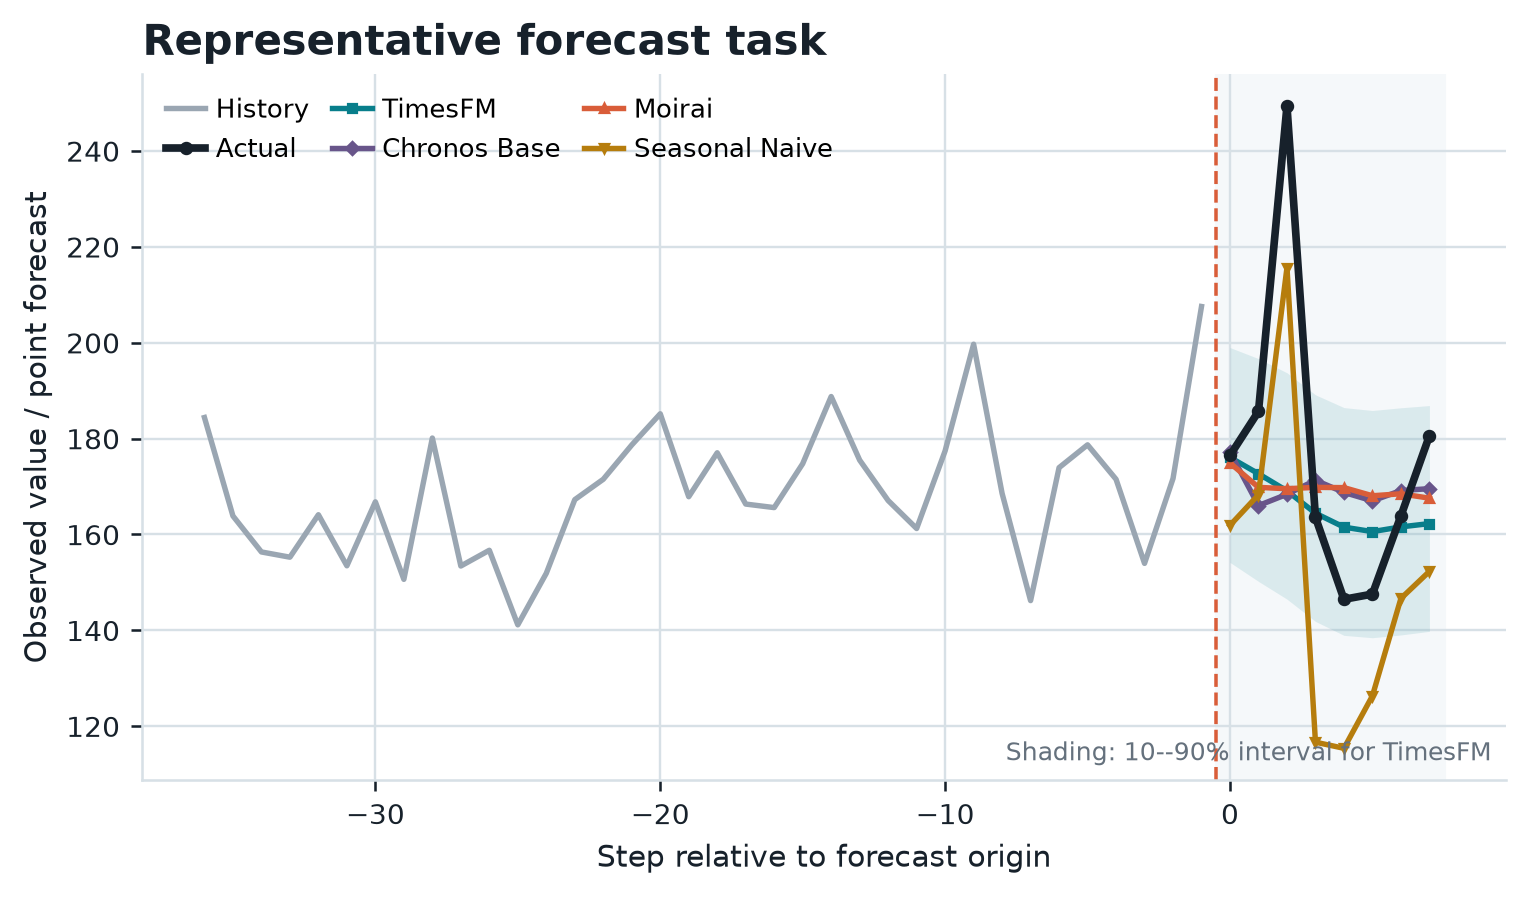
\includegraphics[width=\linewidth,height=4.85cm,keepaspectratio]{nn5-crps-mcs-forecast.png}
    \end{column}
    \begin{column}{0.39\linewidth}
      \centering
      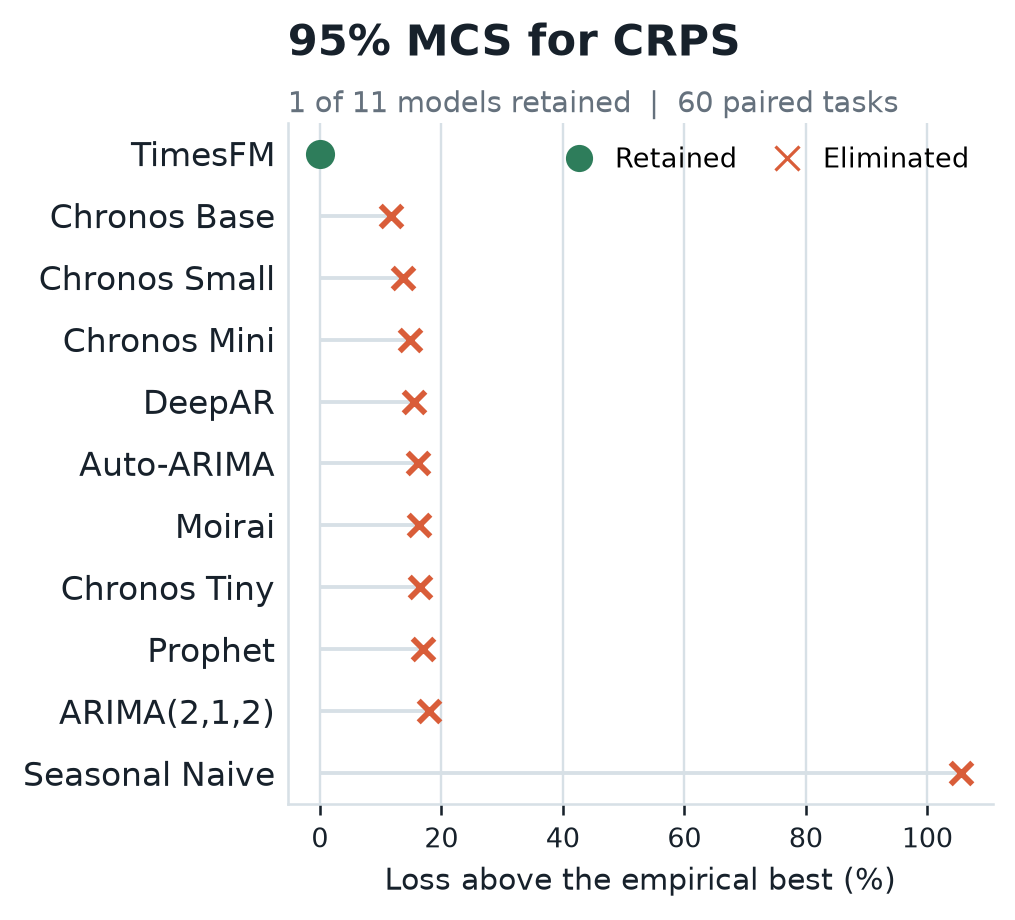
\includegraphics[width=\linewidth,height=4.85cm,keepaspectratio]{nn5-crps-mcs-mcs.png}
    \end{column}
  \end{columns}

  \vspace{0.03cm}
  \begin{center}
    \fontsize{7.6}{8.6}\selectfont
    TimesFM has the lowest CRPS and is the only model retained. In this task,
    its predictive interval covers most of the realized path, although the
    central forecast misses the early spike.
  \end{center}
\end{frame}

% -----------------------------------------------------------------------------
\begin{frame}{M1 Yearly: WQL leaves all models in the MCS}
  \vspace{-0.03cm}
  \begin{columns}[T,totalwidth=0.98\linewidth]
    \begin{column}{0.59\linewidth}
      \centering
      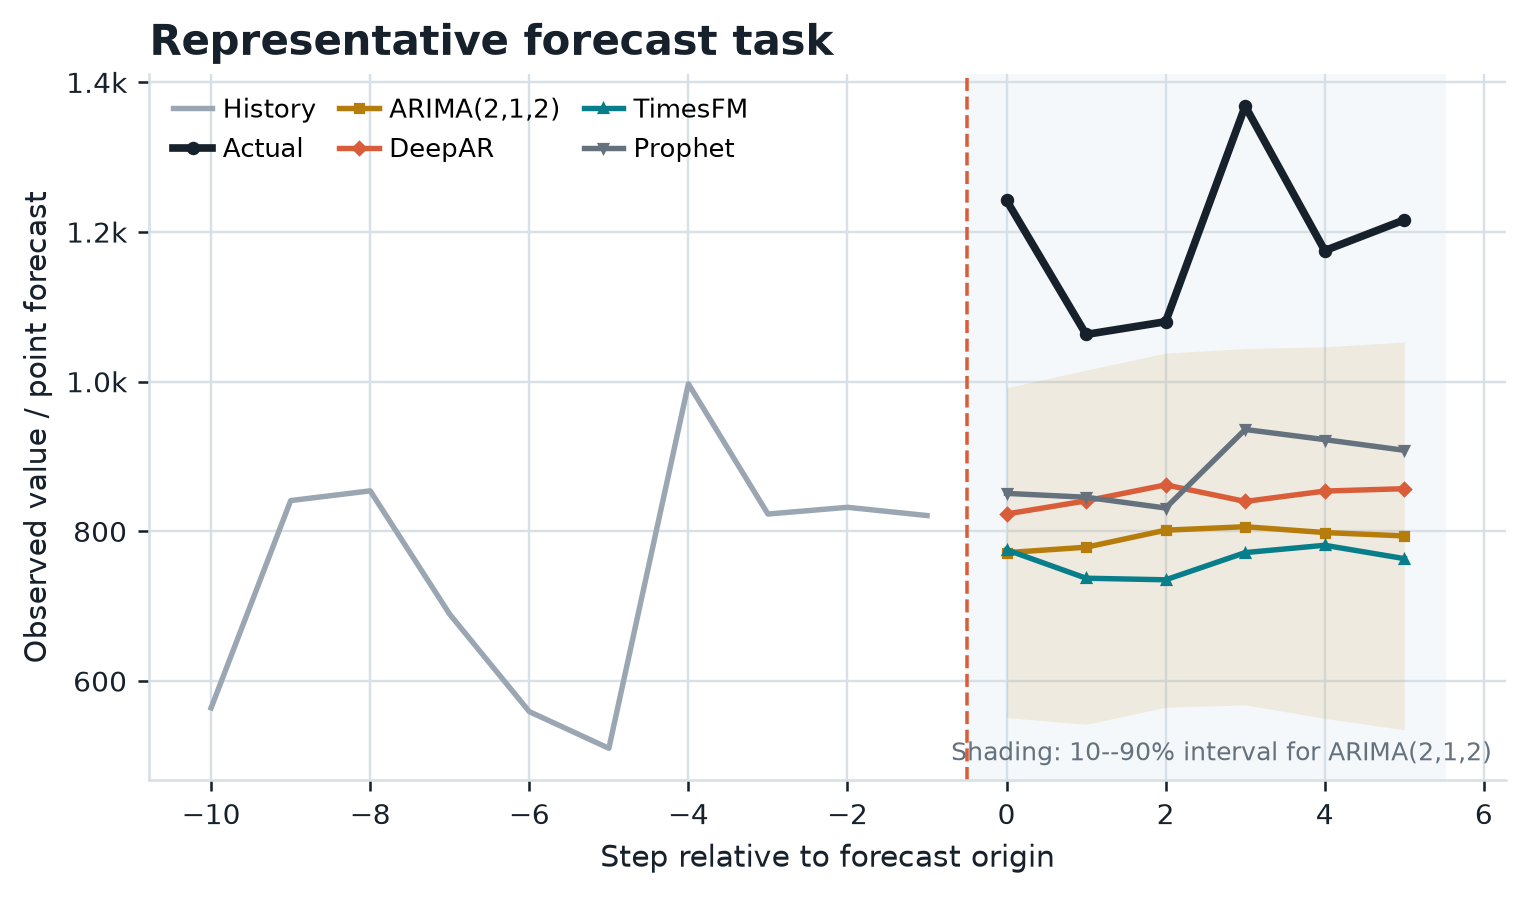
\includegraphics[width=\linewidth,height=4.85cm,keepaspectratio]{m1-wql-mcs-forecast.png}
    \end{column}
    \begin{column}{0.39\linewidth}
      \centering
      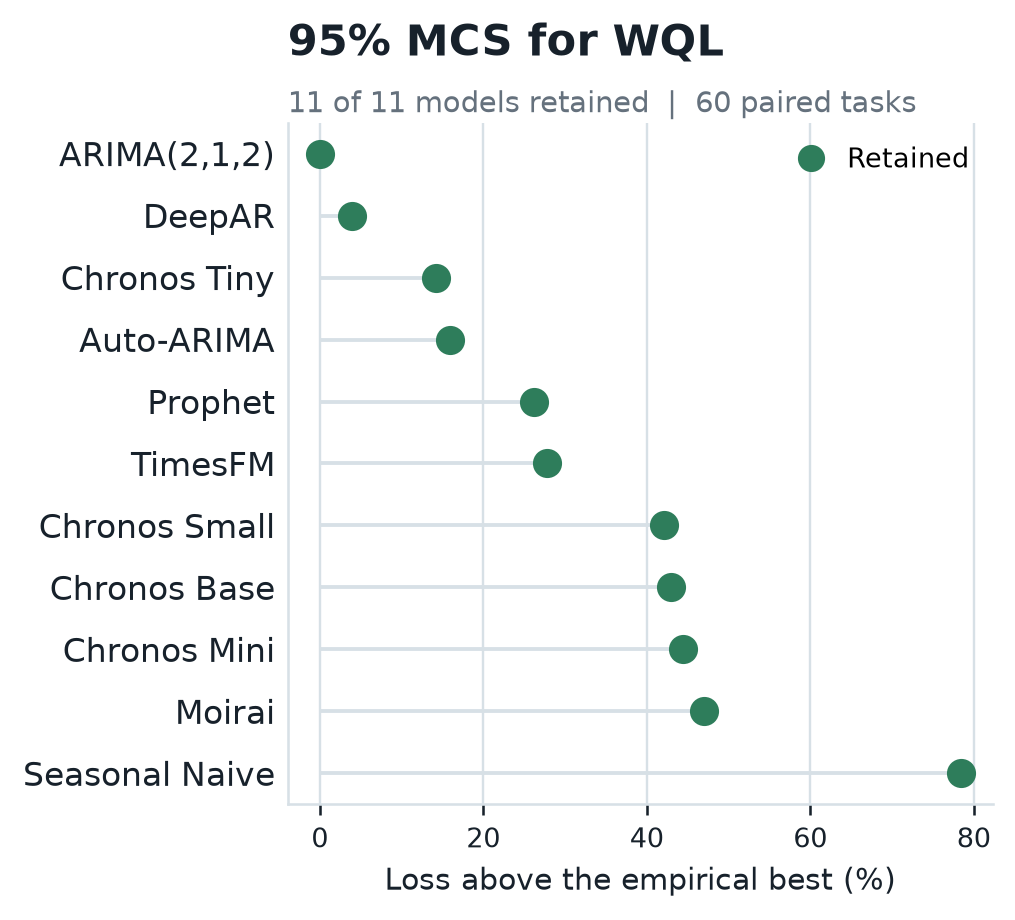
\includegraphics[width=\linewidth,height=4.85cm,keepaspectratio]{m1-wql-mcs-mcs.png}
    \end{column}
  \end{columns}

  \vspace{0.03cm}
  \begin{center}
    \fontsize{7.6}{8.6}\selectfont
    ARIMA records the lowest aggregate WQL, but the MCS cannot eliminate any
    alternative. A first-place empirical rank is therefore not a uniquely
    supported winner on this dataset.
  \end{center}
\end{frame}

% -----------------------------------------------------------------------------
\begin{frame}{Elexon Demand: WQL narrows the MCS to two models}
  \vspace{-0.03cm}
  \begin{columns}[T,totalwidth=0.98\linewidth]
    \begin{column}{0.59\linewidth}
      \centering
      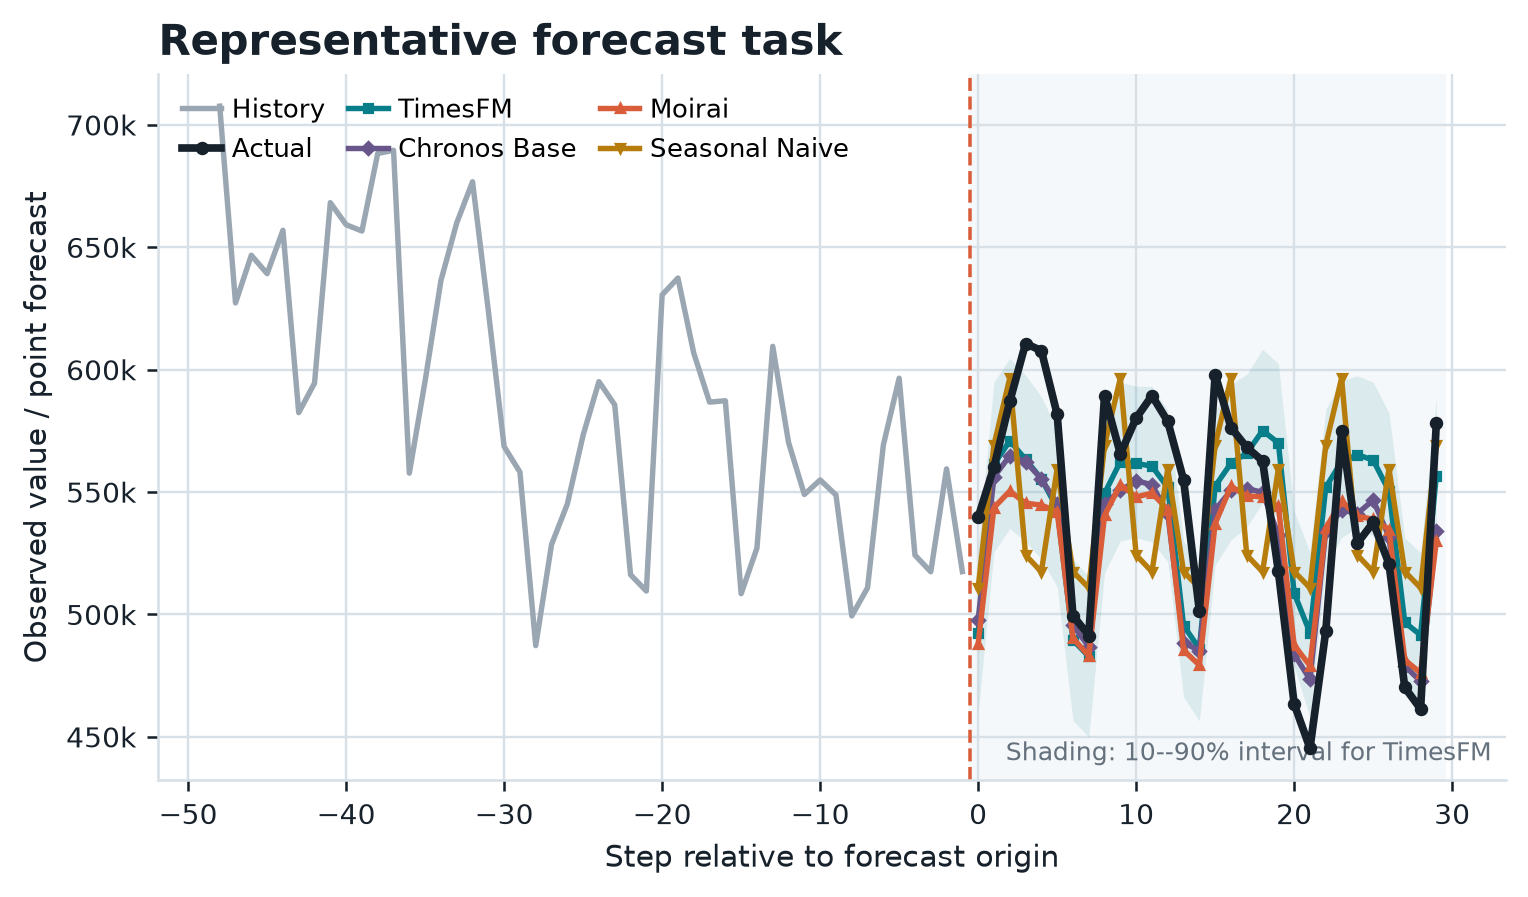
\includegraphics[width=\linewidth,height=4.85cm,keepaspectratio]{elexon-wql-mcs-forecast.png}
    \end{column}
    \begin{column}{0.39\linewidth}
      \centering
      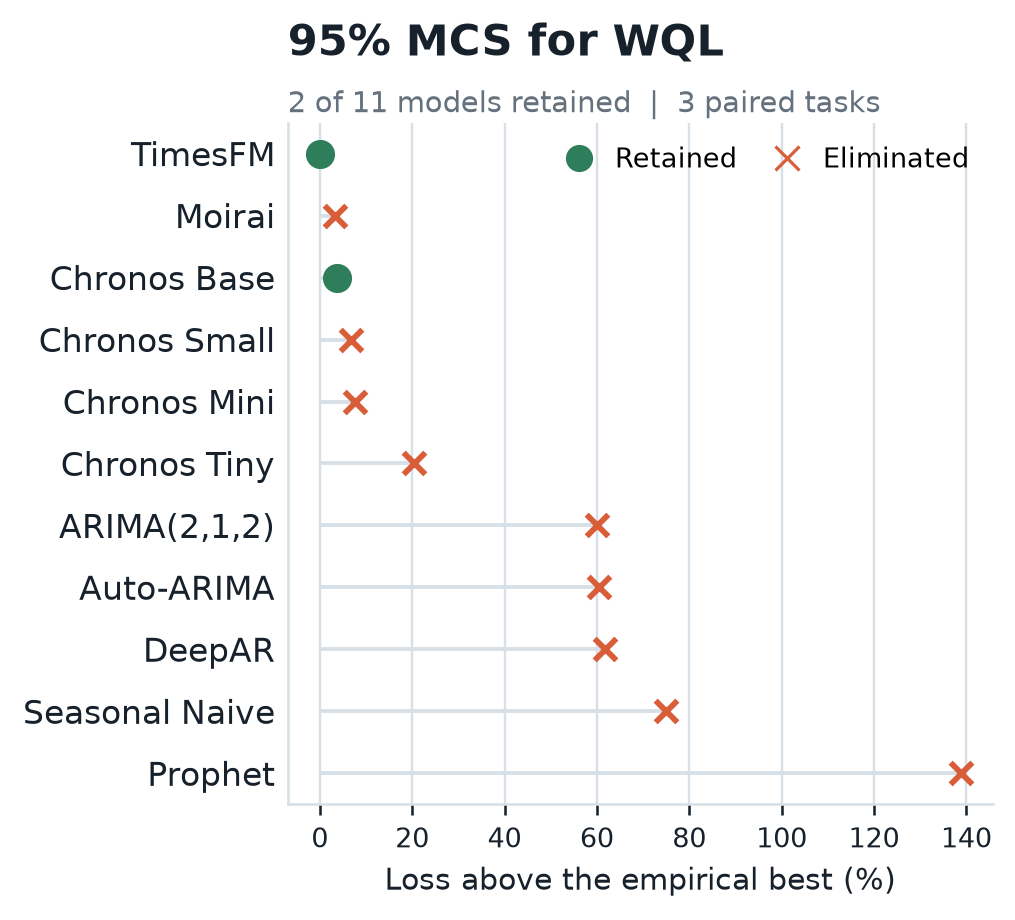
\includegraphics[width=\linewidth,height=4.85cm,keepaspectratio]{elexon-wql-mcs-mcs.png}
    \end{column}
  \end{columns}

  \vspace{0.03cm}
  \begin{center}
    \fontsize{7.6}{8.6}\selectfont
    TimesFM and Chronos Base remain in the set. Because Elexon contributes only
    three paired tasks, this narrow MCS should be treated as exploratory rather
    than as broad evidence of separation.
  \end{center}
\end{frame}

% -----------------------------------------------------------------------------
\begin{frame}{Traffic: MASE leaves a competitive set of six}
  \vspace{-0.03cm}
  \begin{columns}[T,totalwidth=0.98\linewidth]
    \begin{column}{0.59\linewidth}
      \centering
      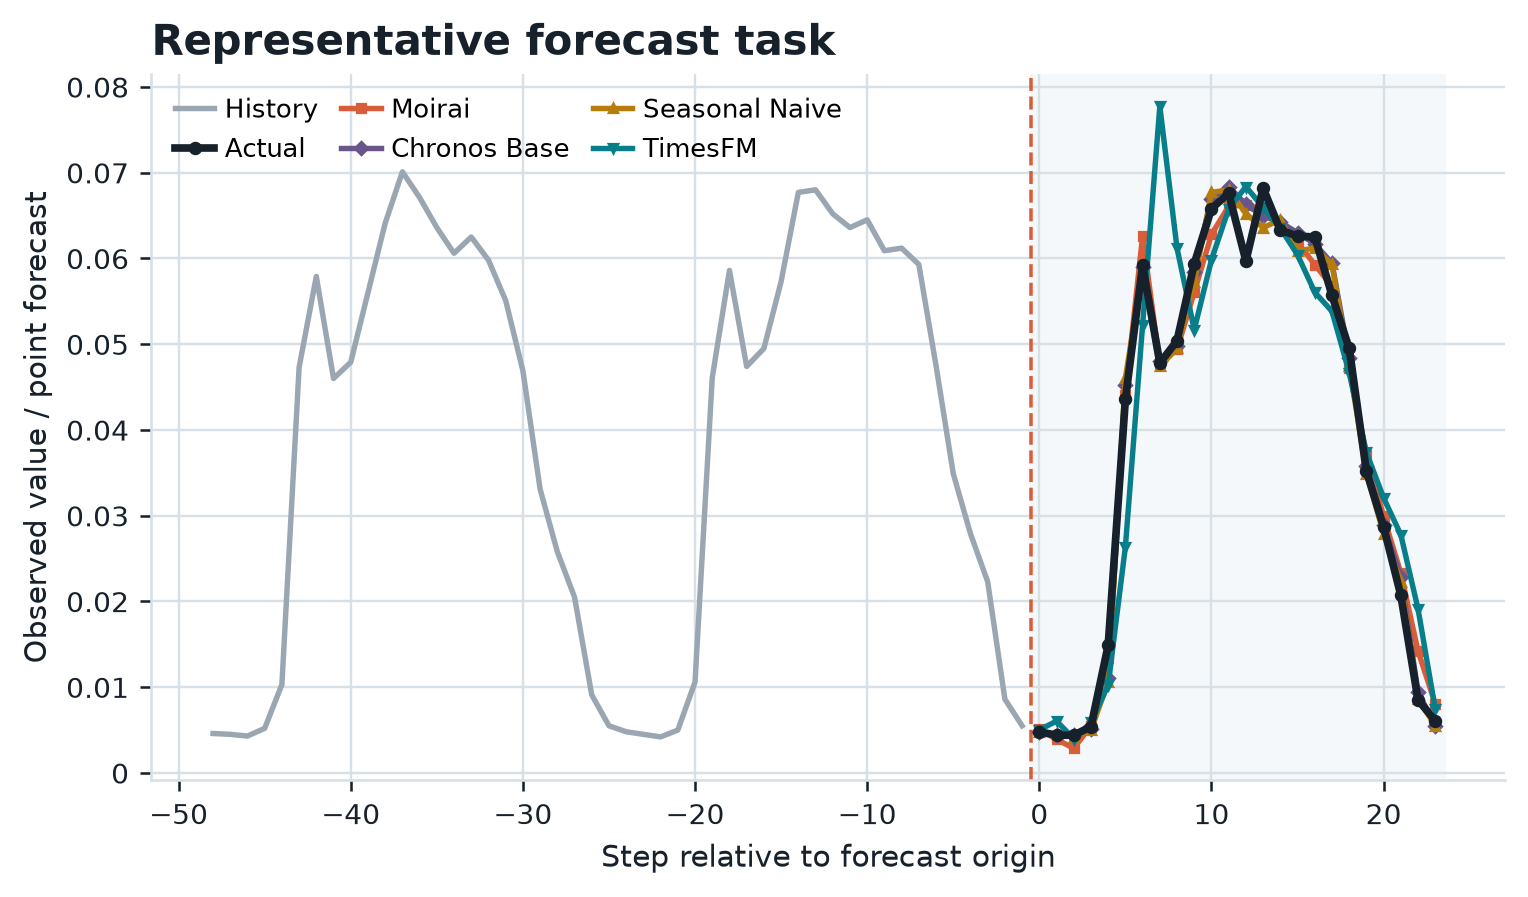
\includegraphics[width=\linewidth,height=4.85cm,keepaspectratio]{traffic-mase-mcs-forecast.png}
    \end{column}
    \begin{column}{0.39\linewidth}
      \centering
      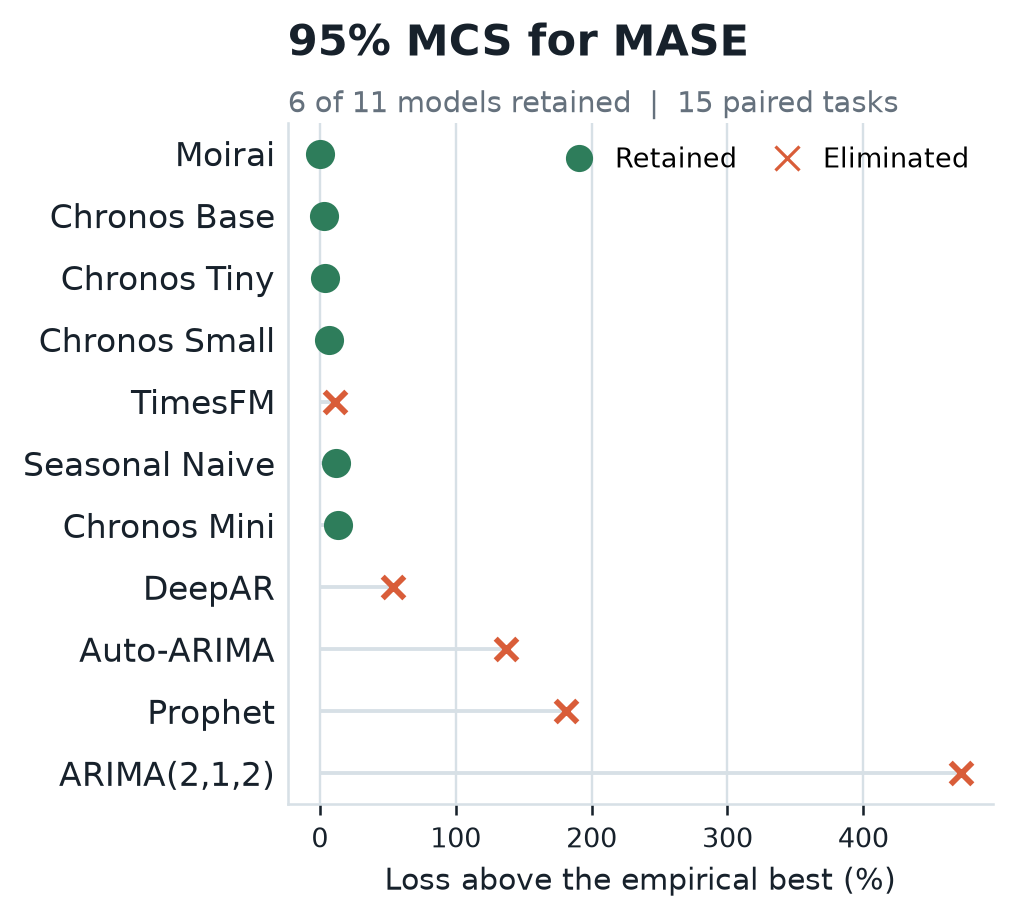
\includegraphics[width=\linewidth,height=4.85cm,keepaspectratio]{traffic-mase-mcs-mcs.png}
    \end{column}
  \end{columns}

  \vspace{0.03cm}
  \begin{center}
    \fontsize{7.6}{8.6}\selectfont
    Moirai has the lowest aggregate MASE, while six models remain. MCS
    membership is determined by paired loss differences, so it need not follow
    the aggregate ranking exactly.
  \end{center}
\end{frame}

% -----------------------------------------------------------------------------
\begin{frame}{Conclusion: empirical results}
  \vspace{0.04cm}
  \begin{columns}[T,totalwidth=0.92\linewidth]
    \begin{column}{0.28\linewidth}
      \colorbox{TealLight}{\parbox{0.90\linewidth}{\centering
        \fontsize{15}{17}\selectfont\bfseries 11 of 12\par
        \scriptsize foundation winner for MASE}}
    \end{column}
    \begin{column}{0.28\linewidth}
      \colorbox{PurpleLight}{\parbox{0.90\linewidth}{\centering
        \fontsize{15}{17}\selectfont\bfseries 11 of 12\par
        \scriptsize foundation winner for WQL}}
    \end{column}
    \begin{column}{0.28\linewidth}
      \colorbox{GreenLight}{\parbox{0.90\linewidth}{\centering
        \fontsize{15}{17}\selectfont\bfseries 11 of 12\par
        \scriptsize foundation winner for CRPS}}
    \end{column}
  \end{columns}

  \vspace{0.20cm}
  \begin{columns}[T,totalwidth=0.93\linewidth]
    \begin{column}{0.46\linewidth}
      \tagbox{PurpleLight}{\textbf{Main pattern}}
      \vspace{0.10cm}

      \fontsize{8.4}{9.8}\selectfont
      \begin{itemize}\setlength{\itemsep}{0.10cm}
        \item A foundation model has the lowest loss in 33 of the 36
          dataset and metric comparisons.
        \item Foundation models win all three metrics on 10 of the 12
          datasets.
        \item They lead on seasonal and higher-frequency data such as M4
          Hourly, NN5 Weekly, Traffic, and Elexon Demand.
        \item TimesFM wins 17 comparisons and Moirai wins 9.
      \end{itemize}
    \end{column}

    \begin{column}{0.40\linewidth}
      \tagbox{GoldLight}{\textbf{The three classical wins}}
      \vspace{0.12cm}

      \fontsize{8.1}{9.3}\selectfont
      \renewcommand{\arraystretch}{1.28}
      \setlength{\tabcolsep}{2.5pt}
      \begin{tabular}{L{1.95cm} C{0.85cm} L{2.00cm}}
        \toprule
        \textbf{Dataset} & \textbf{Metric} & \textbf{Winner} \\
        \midrule
        M1 Yearly & WQL & ARIMA \\
        \rowcolor{Paper} M1 Yearly & CRPS & ARIMA \\
        BLS Macro & MASE & Auto-ARIMA \\
        \bottomrule
      \end{tabular}

      \vspace{0.18cm}
      \fontsize{8.2}{9.5}\selectfont
      Classical methods are most competitive on the economic datasets with
      long trends and changes in level.
    \end{column}
  \end{columns}
\end{frame}

% -----------------------------------------------------------------------------
\begin{frame}{Conclusion: Model Confidence Set results}
  \vspace{0.04cm}
  \begin{columns}[T,totalwidth=0.92\linewidth]
    \begin{column}{0.28\linewidth}
      \colorbox{TealLight}{\parbox{0.90\linewidth}{\centering
        \fontsize{15}{17}\selectfont\bfseries 4 of 12\par
        \scriptsize meaningful comparison for MASE}}
    \end{column}
    \begin{column}{0.28\linewidth}
      \colorbox{PurpleLight}{\parbox{0.90\linewidth}{\centering
        \fontsize{15}{17}\selectfont\bfseries 8 of 12\par
        \scriptsize meaningful comparison for WQL}}
    \end{column}
    \begin{column}{0.28\linewidth}
      \colorbox{GreenLight}{\parbox{0.90\linewidth}{\centering
        \fontsize{15}{17}\selectfont\bfseries 7 of 12\par
        \scriptsize meaningful comparison for CRPS}}
    \end{column}
  \end{columns}

  \vspace{0.20cm}
  \begin{columns}[T,totalwidth=0.93\linewidth]
    \begin{column}{0.46\linewidth}
      \tagbox{PurpleLight}{\textbf{Main pattern}}
      \vspace{0.10cm}

      \fontsize{8.2}{9.5}\selectfont
      \begin{itemize}\setlength{\itemsep}{0.10cm}
        \item The best model from the other family is excluded in 19 of the 36
          comparisons.
        \item WQL and CRPS account for 15 of these 19 results. MASE accounts
          for only 4.
        \item The strongest pattern appears on recurring demand and on sparse
          or noisy series.
        \item Only four comparisons leave one model: all three NN5 losses and
          Weather CRPS.
      \end{itemize}
    \end{column}

    \begin{column}{0.40\linewidth}
      \tagbox{GreenLight}{\textbf{Meaningful on all three losses}}
      \vspace{0.12cm}

      \fontsize{8.1}{9.3}\selectfont
      \renewcommand{\arraystretch}{1.24}
      \setlength{\tabcolsep}{3.5pt}
      \begin{tabular}{L{1.90cm} C{0.85cm} C{0.85cm} C{0.85cm}}
        \toprule
        \textbf{Dataset} & \textbf{MASE} & \textbf{WQL} & \textbf{CRPS} \\
        \midrule
        NN5 Weekly & 1 & 1 & 1 \\
        \rowcolor{Paper} PSM & 7 & 7 & 7 \\
        Elexon Demand & 3 & 2 & 2 \\
        \bottomrule
      \end{tabular}

      \vspace{0.13cm}
      \fontsize{7.9}{9.1}\selectfont
      The table reports the full MCS size. M1 Yearly, BLS Macro, and USGS
      Streamflow do not exclude the other-family winner for any loss.
    \end{column}
  \end{columns}

  \vspace{0.10cm}
  \begin{center}\small\bfseries
    MCS evidence is stronger for WQL and CRPS than for MASE, especially on
    recurring demand and sparse or noisy series.
  \end{center}
\end{frame}

% -----------------------------------------------------------------------------
\begin{frame}{Future work}
  \vspace{0.02cm}
  \begin{columns}[T,totalwidth=0.94\linewidth]
    \begin{column}{0.44\linewidth}
      \colorbox{TealLight}{\parbox{0.92\linewidth}{
        \textbf{Use more datasets}\par\vspace{0.06cm}
        \fontsize{8.1}{9.4}\selectfont
        Add more datasets for each frequency and domain. This would let us test
        whether model families behave differently on seasonal, sparse,
        high-frequency, or trend-dominated data.}}

      \vspace{0.18cm}
      \colorbox{GoldLight}{\parbox{0.92\linewidth}{
        \textbf{Build stronger classical and hybrid models}\par\vspace{0.06cm}
        \fontsize{8.1}{9.4}\selectfont
        Remove trend or seasonality first, forecast the residual with another
        model, and then add the components back. Compare STL with ARIMA or ETS,
        model ensembles, and classical plus foundation-model hybrids.}}
    \end{column}

    \begin{column}{0.44\linewidth}
      \colorbox{PurpleLight}{\parbox{0.92\linewidth}{
        \textbf{Measure the data characteristics}\par\vspace{0.06cm}
        \fontsize{8.1}{9.4}\selectfont
        Use the Pettitt test for level changes, trend tests, seasonality
        strength, autocorrelation, and the share of zero values. Relate these
        measurements to the loss differences between model families.}}

      \vspace{0.18cm}
      \colorbox{GreenLight}{\parbox{0.92\linewidth}{
        \textbf{Strengthen the statistical analysis}\par\vspace{0.06cm}
        \fontsize{8.1}{9.4}\selectfont
        Add more rolling forecast origins. Use hierarchical models across
        datasets and series, and check how the MCS changes with different
        bootstrap blocks and significance levels.}}
    \end{column}
  \end{columns}

  \vspace{0.19cm}
  \begin{center}
    \tagbox{Paper}{\small\textbf{Goal: choose methods from measurable properties
    of the series, not from one overall ranking.}}
  \end{center}
\end{frame}

% =============================================================================
% Appendix frames do not increment the main presentation slide count.
\appendix
\setbeamertemplate{footline}{%
  \leavevmode
  \hbox to \paperwidth{%
    \hspace{0.68cm}%
    {\usebeamerfont{footline}\color{Muted}Amirhossein Bagheri}%
    \hfill
    {\usebeamerfont{footline}\color{Muted}Forecasting benchmark \quad Appendix}%
    \hspace{0.40cm}%
  }
  \vspace{0.16cm}
}

% -----------------------------------------------------------------------------
\begin{frame}[noframenumbering]{Appendix: how large is the family-level advantage?}
  \vspace{0.01cm}
  \begin{center}
    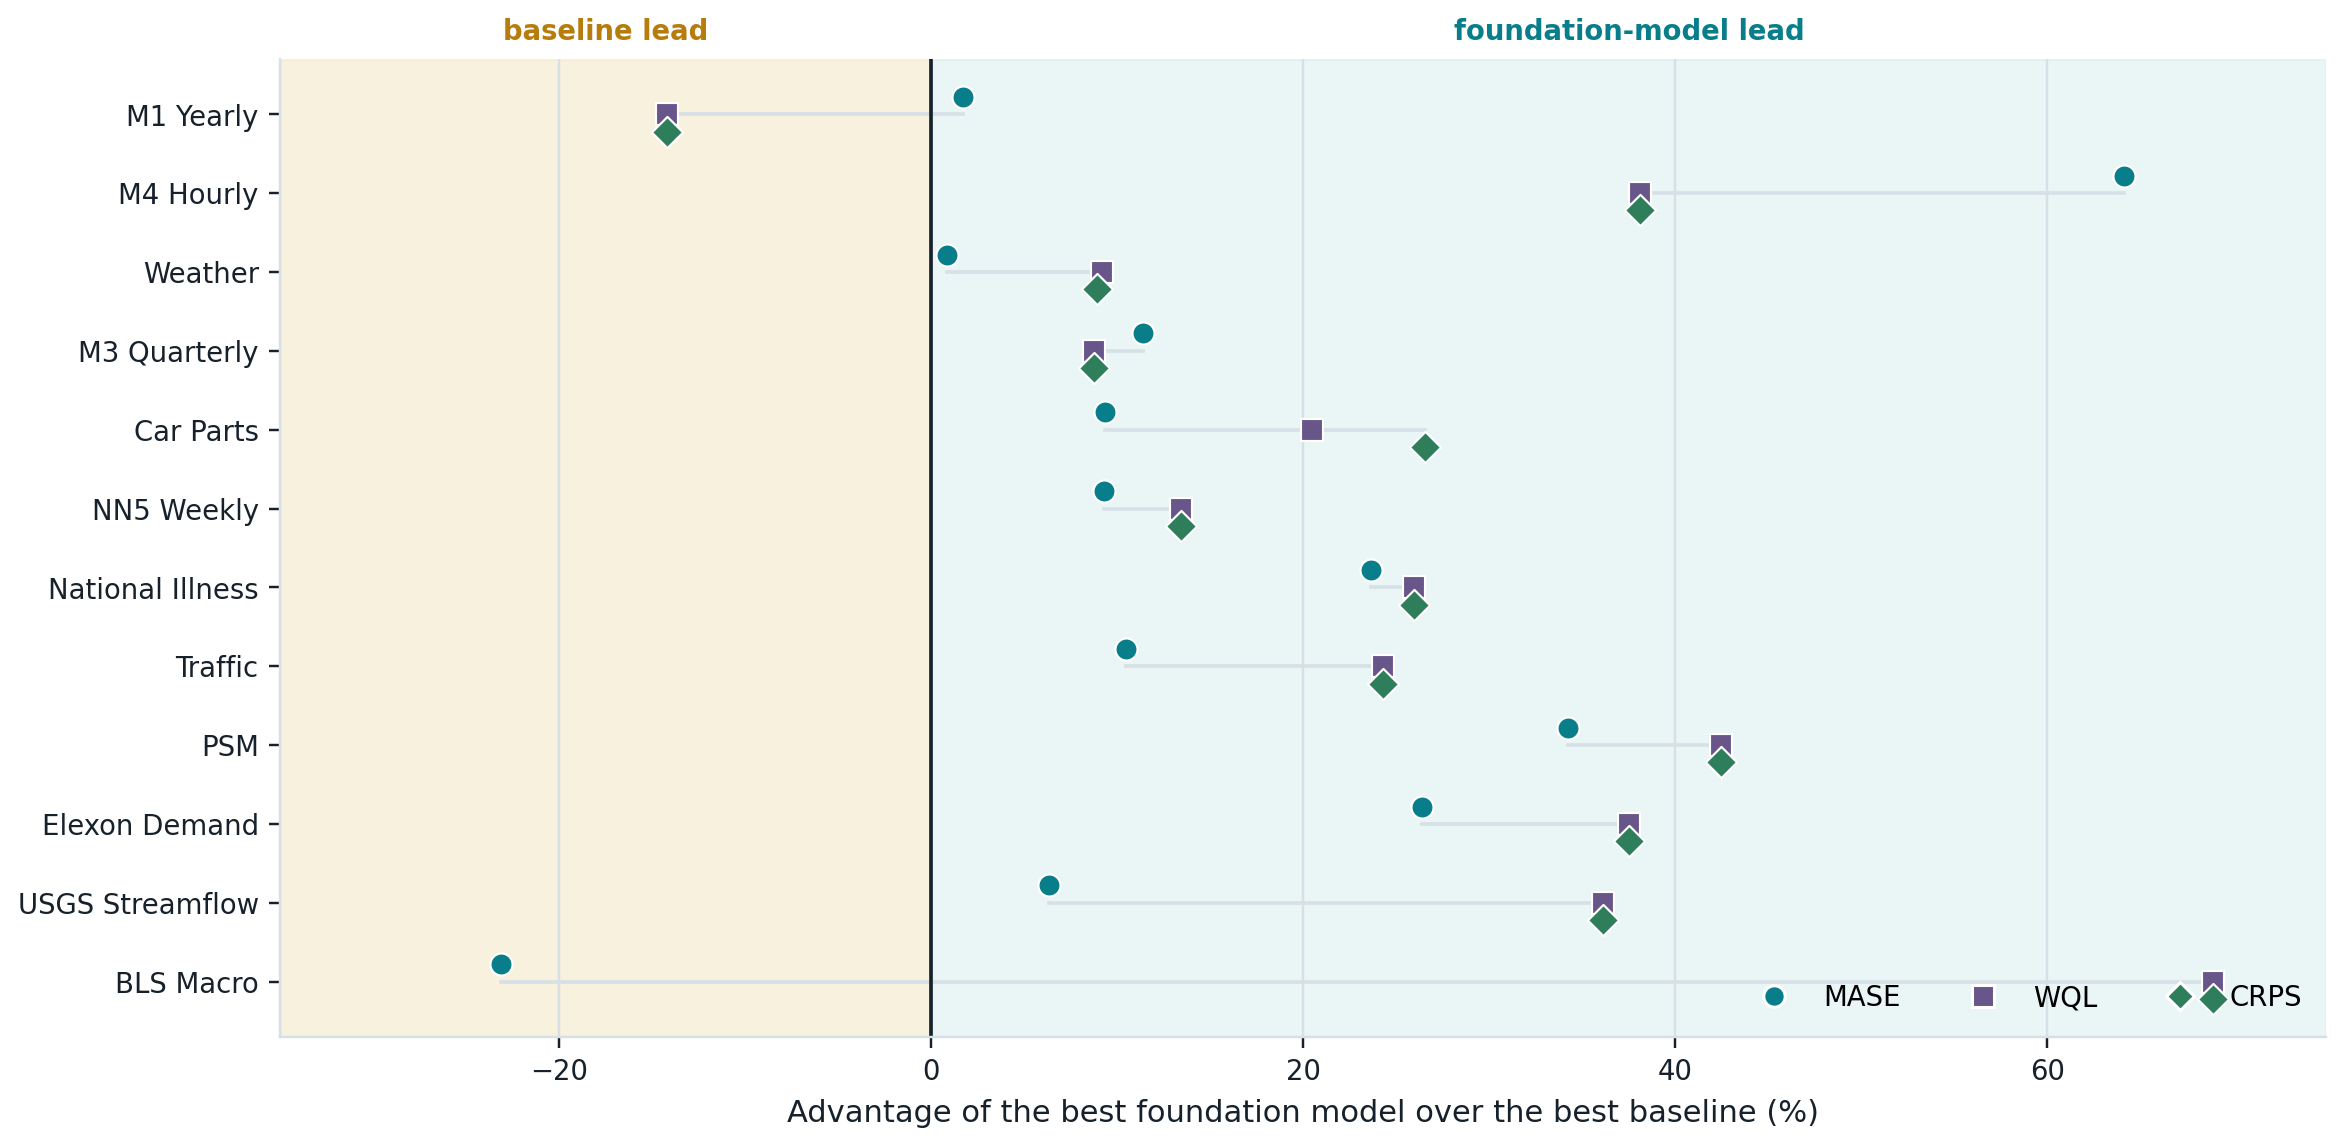
\includegraphics[width=0.96\linewidth,height=5.25cm,keepaspectratio]{appendix-family-loss-gap.png}

    \vspace{0.08cm}
    \colorbox{TealLight}{\parbox{0.90\linewidth}{\centering\scriptsize
      Foundation models lead in 33 of 36 comparisons, but the margin varies
      sharply. The three baseline wins are M1 Yearly WQL and CRPS, and BLS
      Macro MASE.}}
  \end{center}
\end{frame}

% -----------------------------------------------------------------------------
\begin{frame}[noframenumbering]{Appendix: rank consistency across datasets and losses}
  \vspace{0.01cm}
  \begin{center}
    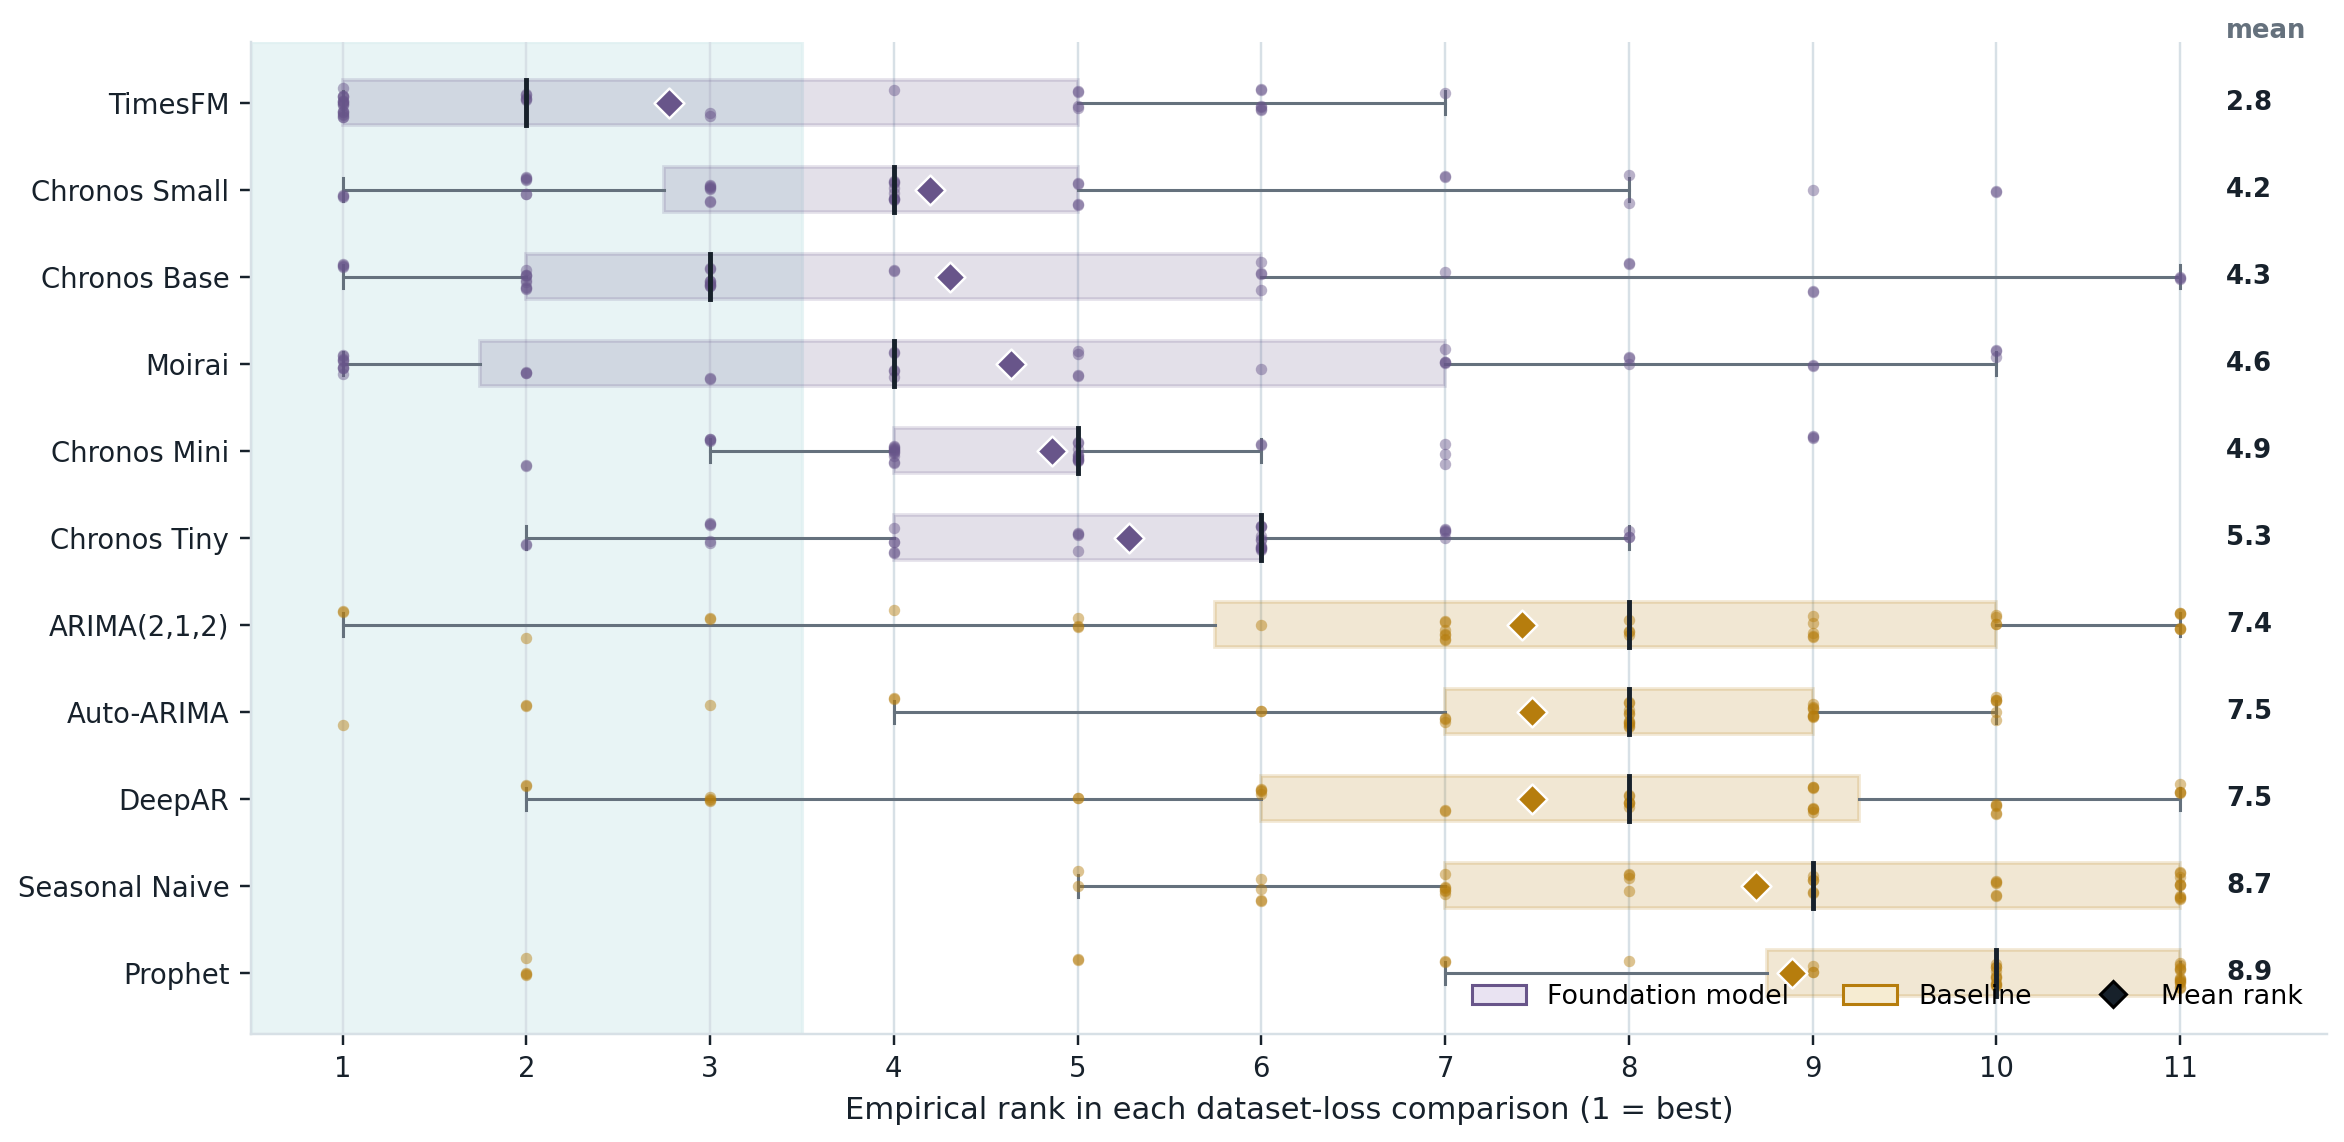
\includegraphics[width=0.96\linewidth,height=5.25cm,keepaspectratio]{appendix-rank-distribution.png}

    \vspace{0.08cm}
    \colorbox{PurpleLight}{\parbox{0.90\linewidth}{\centering\scriptsize
      TimesFM has the best mean rank and the most consistently strong placement.
      The other foundation-model variants move more across datasets.}}
  \end{center}
\end{frame}

% -----------------------------------------------------------------------------
\begin{frame}[noframenumbering]{Appendix: where is the 95\% MCS selective?}
  \vspace{0.01cm}
  \begin{center}
    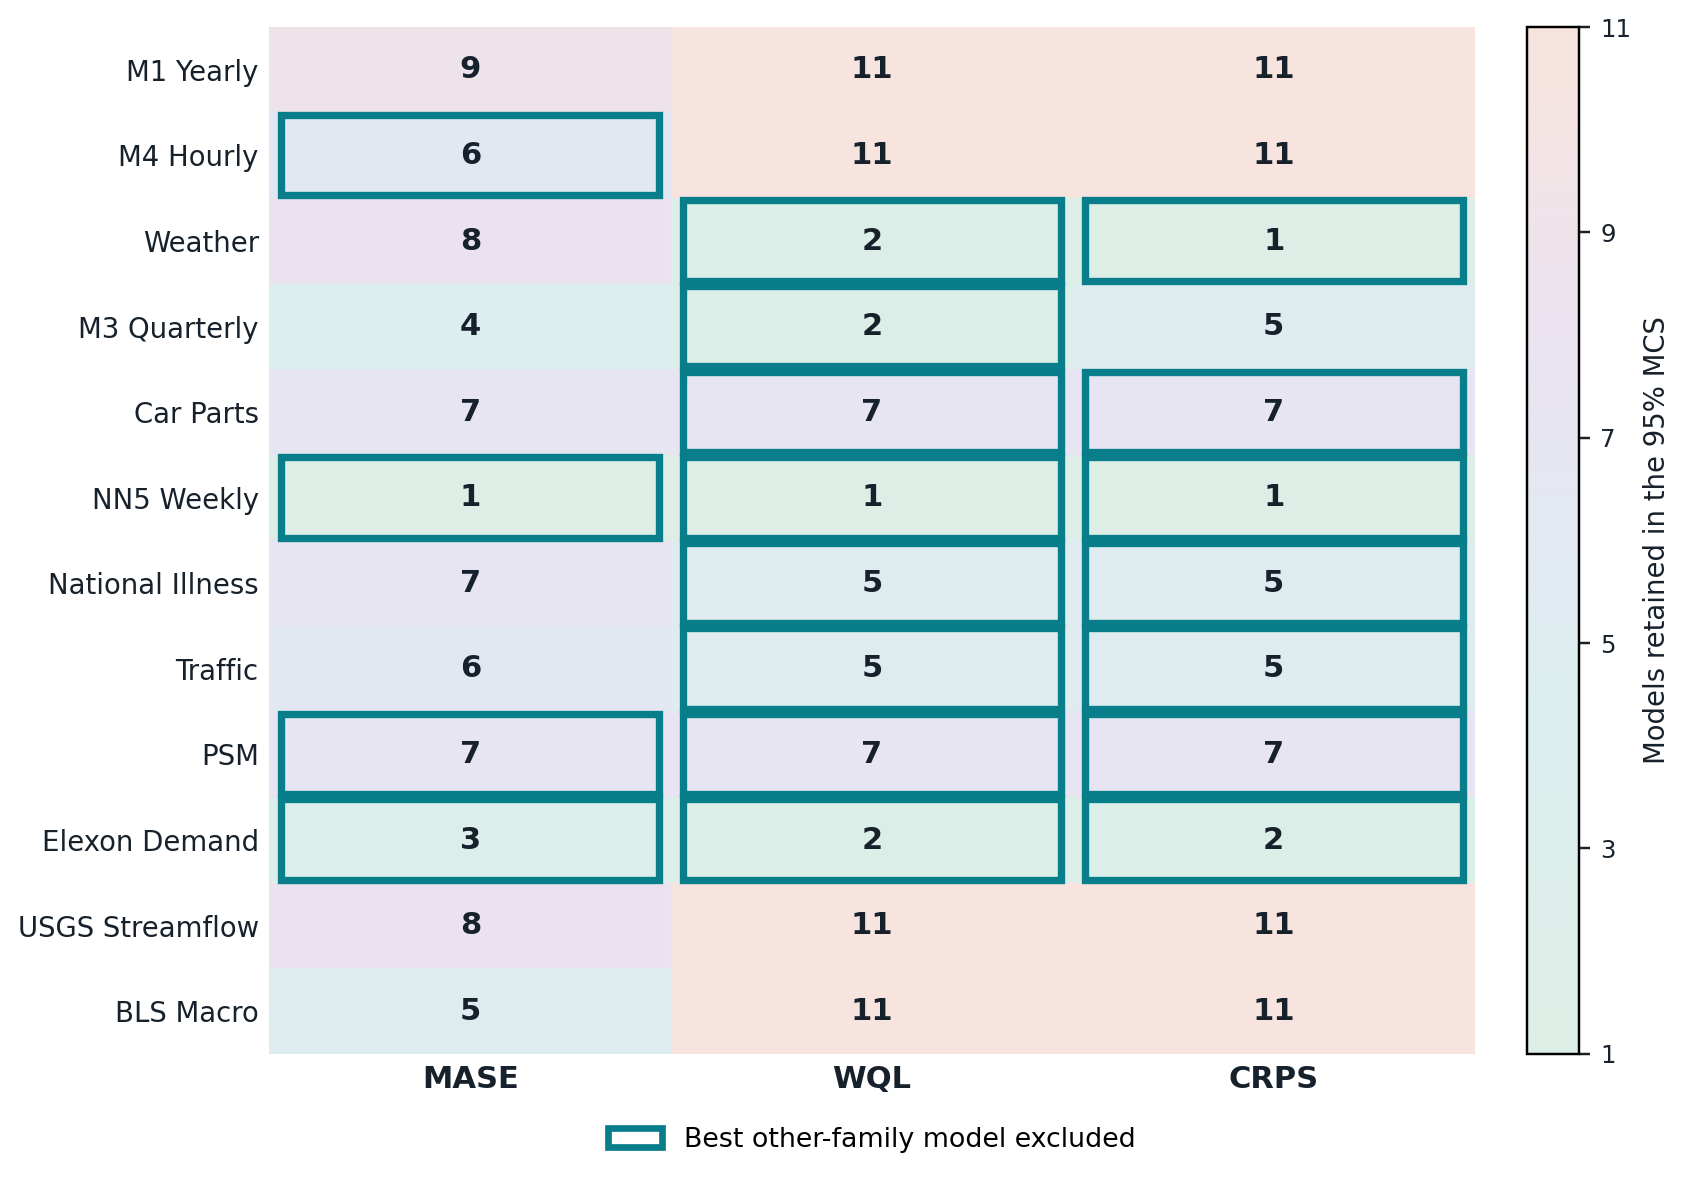
\includegraphics[width=0.82\linewidth,height=5.30cm,keepaspectratio]{appendix-mcs-size-heatmap.png}

    \vspace{0.05cm}
    \colorbox{GreenLight}{\parbox{0.90\linewidth}{\centering\scriptsize
      NN5 produces a one-model set for every loss. Several datasets retain many
      models even when their empirical winner is a foundation model.}}
  \end{center}
\end{frame}

% -----------------------------------------------------------------------------
\begin{frame}[noframenumbering]{Appendix: calibration of the 80\% prediction interval}
  \vspace{0.01cm}
  \begin{center}
    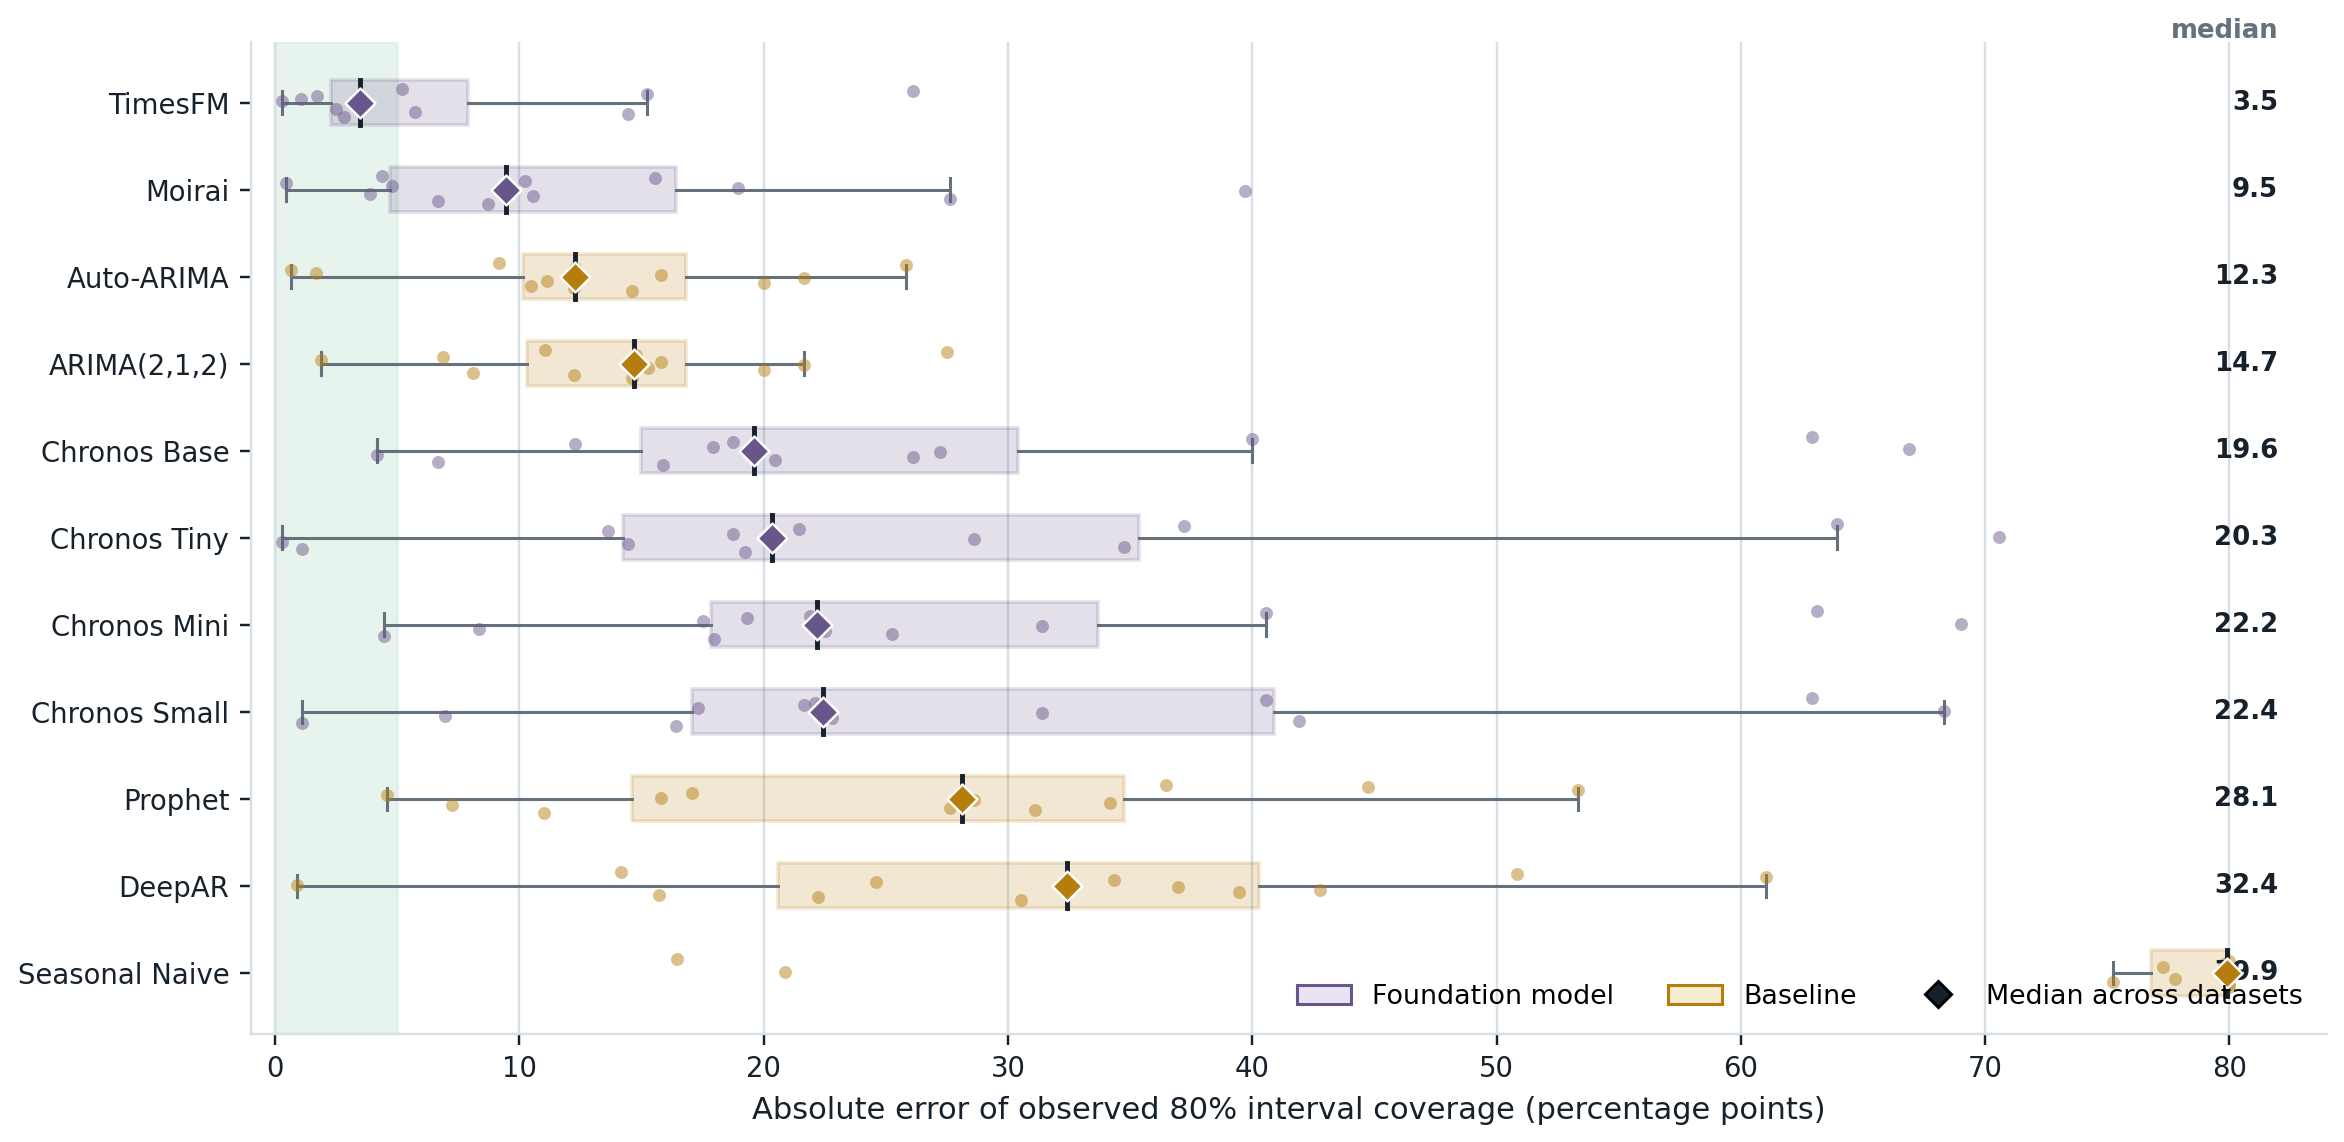
\includegraphics[width=0.96\linewidth,height=5.25cm,keepaspectratio]{appendix-calibration-distribution.png}

    \vspace{0.08cm}
    \colorbox{GoldLight}{\parbox{0.90\linewidth}{\centering\scriptsize
      TimesFM has the smallest median coverage error across datasets. Coverage
      alone is not enough: WQL and CRPS also reward narrower, sharper forecasts.}}
  \end{center}
\end{frame}

% -----------------------------------------------------------------------------
\begin{frame}[noframenumbering]{Appendix: recorded runtime versus empirical rank}
  \vspace{0.01cm}
  \begin{center}
    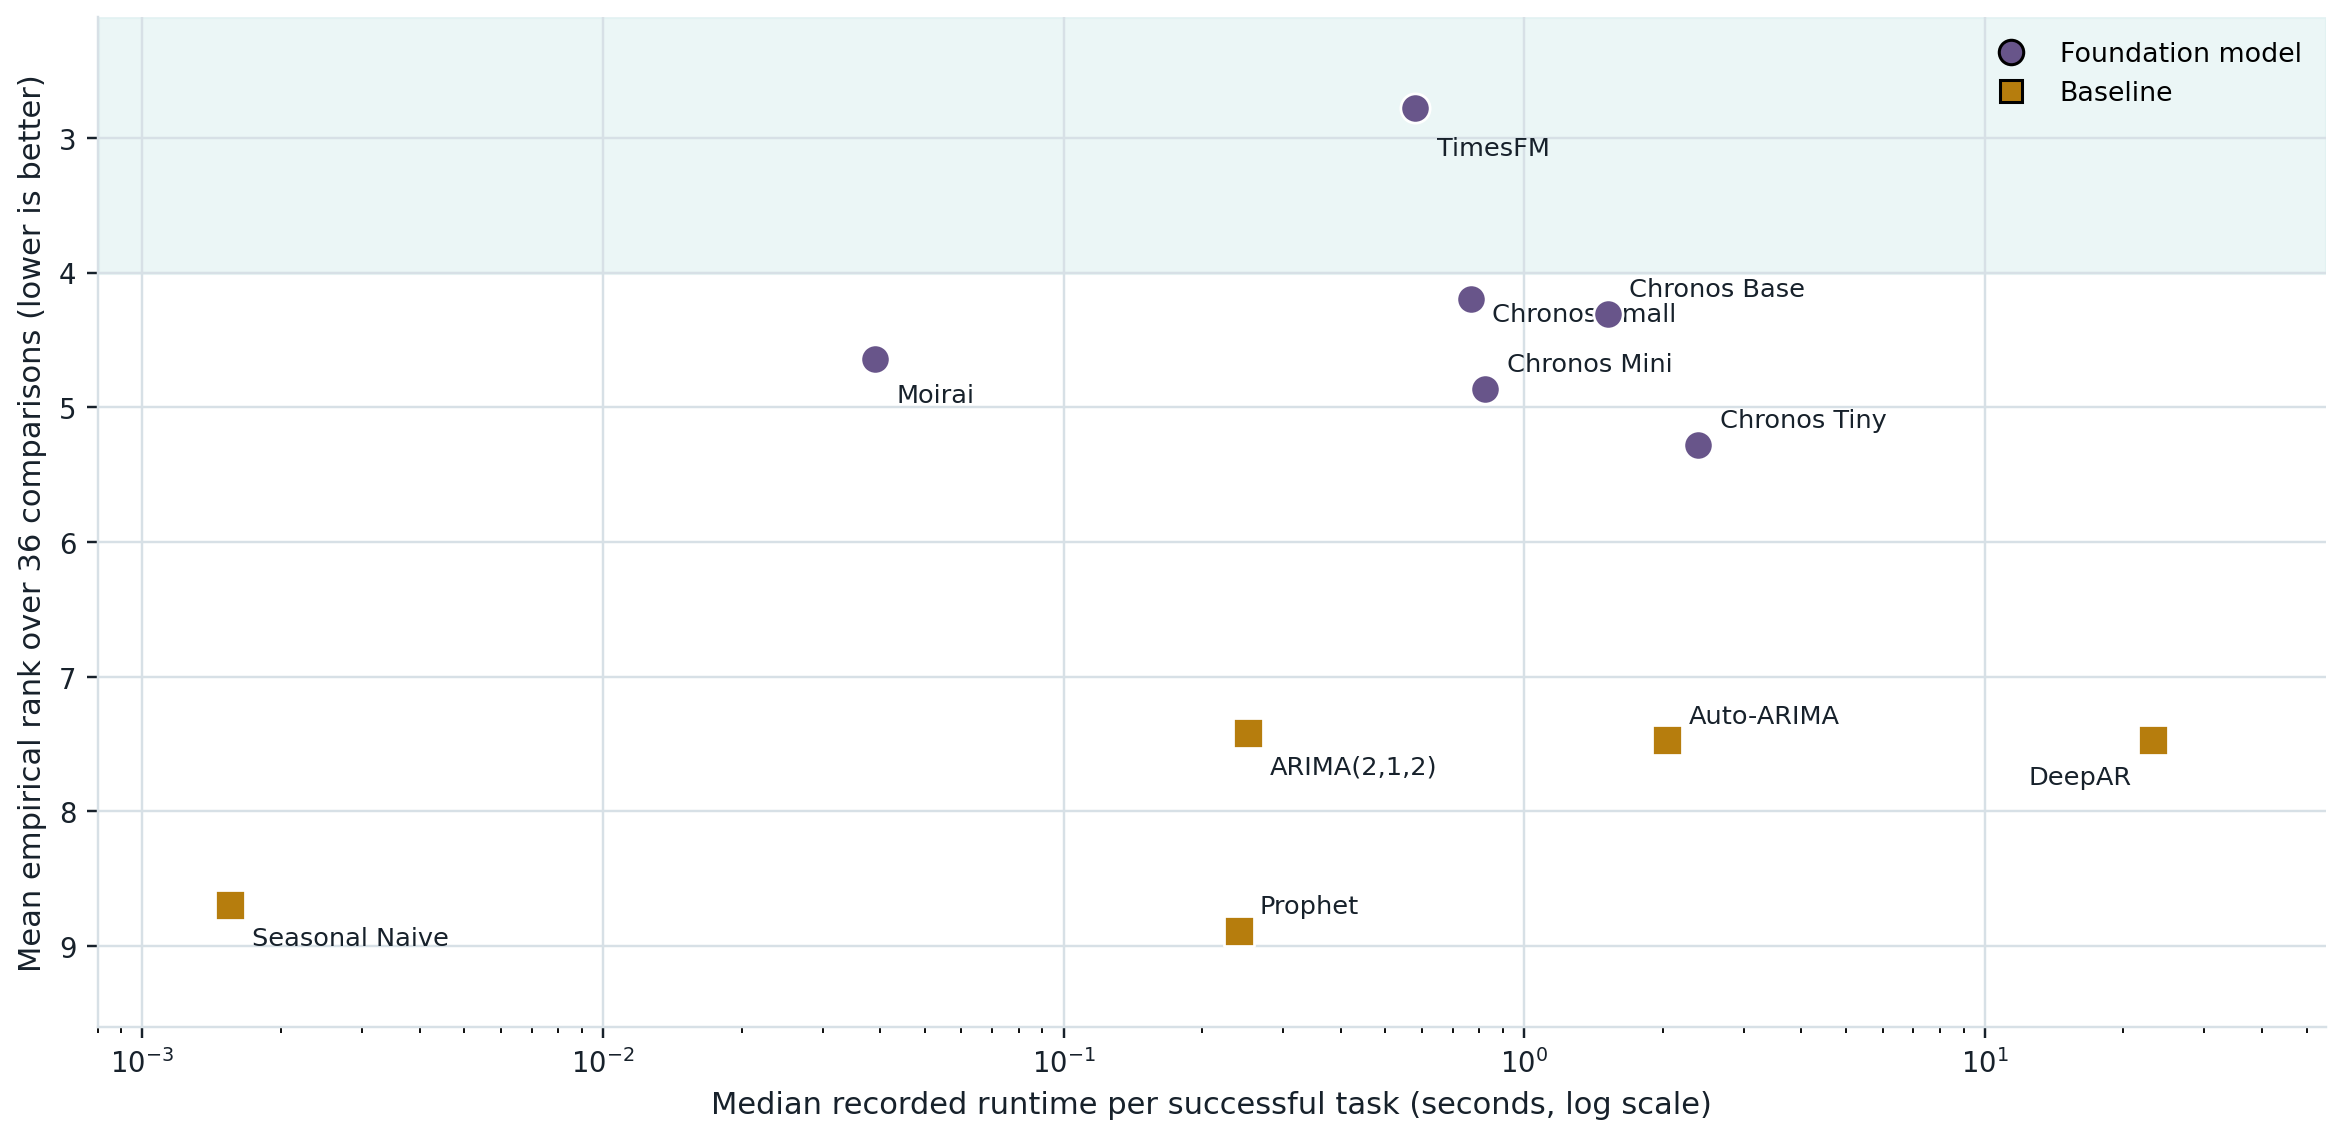
\includegraphics[width=0.96\linewidth,height=5.25cm,keepaspectratio]{appendix-speed-accuracy.png}

    \vspace{0.08cm}
    \colorbox{Paper}{\parbox{0.90\linewidth}{\centering\scriptsize
      TimesFM has the best mean rank; Moirai combines a top-five mean rank with
      low recorded task time. Runtime values are specific to this benchmark setup.}}
  \end{center}
\end{frame}

% -----------------------------------------------------------------------------
\begin{frame}[noframenumbering]{Appendix: paired forecast tasks used by the MCS}
  \vspace{0.03cm}
  \begin{center}
    \fontsize{6.6}{7.4}\selectfont
    \renewcommand{\arraystretch}{1.08}
    \setlength{\tabcolsep}{3.2pt}
    \begin{tabular}{L{2.40cm} L{4.15cm} C{0.80cm} C{1.08cm} C{1.08cm} C{1.08cm} C{1.25cm}}
      \toprule
      \textbf{Dataset} & \textbf{Main pattern} & \textbf{Series} &
      \textbf{MASE} & \textbf{WQL} & \textbf{CRPS} & \textbf{Evidence} \\
      \midrule
      Car Parts & Sparse demand, many zeros & 20 & 39 & 31 & 40 & adequate \\
      \rowcolor{Paper} M1 Yearly & Annual trends and level changes & 20 & 60 & 60 & 60 & adequate \\
      M3 Quarterly & Trend and quarterly cycles & 20 & 60 & 60 & 60 & adequate \\
      \rowcolor{Paper} M4 Hourly & Daily cycles and noise & 20 & 60 & 60 & 60 & adequate \\
      NN5 Weekly & Annual pattern, holidays, demand shifts & 20 & 60 & 60 & 60 & adequate \\
      \rowcolor{Paper} Weather & Zeros and seasonal rainfall & 20 & 60 & 46 & 60 & adequate \\
      National Illness & Annual cycle and sudden peaks & 1 & 3 & 3 & 3 & very low \\
      \rowcolor{Paper} PSM & Anomalies and noisy sensors & 5 & 15 & 15 & 15 & low \\
      Traffic & Daily and weekly cycles & 5 & 15 & 15 & 15 & low \\
      \rowcolor{Paper} BLS Macro & Long trends and structural changes & 3 & 7 & 7 & 7 & very low \\
      Elexon Demand & Weekly cycle and weather effects & 1 & 3 & 3 & 3 & very low \\
      \rowcolor{Paper} USGS Streamflow & Seasonality, extremes, and gaps & 5 & 13 & 13 & 13 & low \\
      \bottomrule
    \end{tabular}
  \end{center}

  \vspace{0.08cm}
  \begin{center}\fontsize{6.5}{7.3}\selectfont\color{Muted}
    A paired task is one series at one forecast origin after averaging the three
    model repetitions. Missing or undefined losses reduce some task counts.
  \end{center}
\end{frame}

% -----------------------------------------------------------------------------
\begin{frame}[noframenumbering]{Appendix: lowest loss and MCS size}
  \vspace{0.02cm}
  \begin{center}
    \fontsize{6.8}{7.6}\selectfont
    \renewcommand{\arraystretch}{1.05}
    \setlength{\tabcolsep}{4.2pt}
    \begin{tabular}{L{2.65cm} C{3.30cm} C{3.30cm} C{3.30cm}}
      \toprule
      \textbf{Dataset} & \textbf{MASE} & \textbf{WQL} & \textbf{CRPS} \\
      \midrule
      Car Parts & \foundationwinner{Moirai (7)} & \foundationwinner{Moirai (7)} & \foundationwinner{Moirai (7)} \\
      \rowcolor{Paper} M1 Yearly & \foundationwinner{TimesFM (9)} & \classicalwinner{ARIMA (11)} & \classicalwinner{ARIMA (11)} \\
      M3 Quarterly & \foundationwinner{TimesFM (4)} & \foundationwinner{TimesFM (2)} & \foundationwinner{TimesFM (5)} \\
      \rowcolor{Paper} M4 Hourly & \foundationwinner{Chronos Base (6)} & \foundationwinner{Chronos Base (11)} & \foundationwinner{Chronos Base (11)} \\
      NN5 Weekly & \foundationwinner{TimesFM (1)} & \foundationwinner{TimesFM (1)} & \foundationwinner{TimesFM (1)} \\
      \rowcolor{Paper} Weather & \foundationwinner{Chronos Base (8)} & \foundationwinner{Moirai (2)} & \foundationwinner{Moirai (1)} \\
      National Illness & \foundationwinner{TimesFM (7)} & \foundationwinner{TimesFM (5)} & \foundationwinner{TimesFM (5)} \\
      \rowcolor{Paper} PSM & \foundationwinner{Chronos Small (7)} & \foundationwinner{Chronos Small (7)} & \foundationwinner{Chronos Small (7)} \\
      Traffic & \foundationwinner{Moirai (6)} & \foundationwinner{Moirai (5)} & \foundationwinner{Moirai (5)} \\
      \rowcolor{Paper} BLS Macro & \classicalwinner{Auto-ARIMA (5)} & \foundationwinner{TimesFM (11)} & \foundationwinner{TimesFM (11)} \\
      Elexon Demand & \foundationwinner{TimesFM (3)} & \foundationwinner{TimesFM (2)} & \foundationwinner{TimesFM (2)} \\
      \rowcolor{Paper} USGS Streamflow & \foundationwinner{Moirai (8)} & \foundationwinner{TimesFM (11)} & \foundationwinner{TimesFM (11)} \\
      \bottomrule
    \end{tabular}
  \end{center}

  \vspace{0.10cm}
  \begin{center}\scriptsize
    Each entry is \textbf{empirical winner (number of models in the 95\% MCS)}.
    \quad \tagbox{PurpleLight}{foundation winner}
    \quad \tagbox{GoldLight}{nonfoundation winner}
  \end{center}
\end{frame}

% -----------------------------------------------------------------------------
\begin{frame}[noframenumbering]{Appendix: who remains in each confidence set?}
  \vspace{0.02cm}
  \begin{center}
    \fontsize{7.0}{7.8}\selectfont
    \renewcommand{\arraystretch}{1.08}
    \setlength{\tabcolsep}{5.4pt}
    \begin{tabular}{L{3.20cm} C{2.95cm} C{2.95cm} C{2.95cm}}
      \toprule
      \textbf{Dataset} & \textbf{MASE} & \textbf{WQL} & \textbf{CRPS} \\
      \midrule
      Car Parts & 6 F + 1 B & 6 F + 1 B & 6 F + 1 B \\
      \rowcolor{Paper} M1 Yearly & 4 F + 5 B & \cellcolor{CoralLight}6 F + 5 B & \cellcolor{CoralLight}6 F + 5 B \\
      M3 Quarterly & 2 F + 2 B & \cellcolor{GreenLight}\textbf{2 F + 0 B} & 3 F + 2 B \\
      \rowcolor{Paper} M4 Hourly & 5 F + 1 B & \cellcolor{CoralLight}6 F + 5 B & \cellcolor{CoralLight}6 F + 5 B \\
      NN5 Weekly & \cellcolor{GreenLight}\textbf{1 F + 0 B} & \cellcolor{GreenLight}\textbf{1 F + 0 B} & \cellcolor{GreenLight}\textbf{1 F + 0 B} \\
      \rowcolor{Paper} Weather & 6 F + 2 B & \cellcolor{GreenLight}\textbf{2 F + 0 B} & \cellcolor{GreenLight}\textbf{1 F + 0 B} \\
      National Illness & 5 F + 2 B & 4 F + 1 B & 4 F + 1 B \\
      \rowcolor{Paper} PSM & 6 F + 1 B & 6 F + 1 B & 6 F + 1 B \\
      Traffic & 5 F + 1 B & \cellcolor{GreenLight}\textbf{5 F + 0 B} & \cellcolor{GreenLight}\textbf{5 F + 0 B} \\
      \rowcolor{Paper} BLS Macro & 2 F + 3 B & \cellcolor{CoralLight}6 F + 5 B & \cellcolor{CoralLight}6 F + 5 B \\
      Elexon Demand & \cellcolor{GreenLight}\textbf{3 F + 0 B} & \cellcolor{GreenLight}\textbf{2 F + 0 B} & \cellcolor{GreenLight}\textbf{2 F + 0 B} \\
      \rowcolor{Paper} USGS Streamflow & 5 F + 3 B & \cellcolor{CoralLight}6 F + 5 B & \cellcolor{CoralLight}6 F + 5 B \\
      \bottomrule
    \end{tabular}
  \end{center}

  \vspace{0.09cm}
  \begin{center}\scriptsize
    F = foundation-model variant; B = nonfoundation baseline.
    Green cells exclude every baseline. Coral cells retain all 11 candidates.
  \end{center}
\end{frame}

% -----------------------------------------------------------------------------
\begin{frame}[noframenumbering]{Appendix: empirical wins by model and loss}
  \vspace{0.05cm}
  \begin{columns}[T,totalwidth=0.92\linewidth]
    \begin{column}{0.53\linewidth}
      \fontsize{8.0}{9.0}\selectfont
      \renewcommand{\arraystretch}{1.18}
      \setlength{\tabcolsep}{5.0pt}
      \begin{tabular}{L{2.30cm} C{0.85cm} C{0.85cm} C{0.85cm} C{0.85cm}}
        \toprule
        \textbf{Model} & \textbf{MASE} & \textbf{WQL} & \textbf{CRPS} & \textbf{Total} \\
        \midrule
        \rowcolor{TealLight} TimesFM & 5 & 6 & 6 & \textbf{17} \\
        Moirai & 3 & 3 & 3 & \textbf{9} \\
        \rowcolor{Paper} Chronos Base & 2 & 1 & 1 & \textbf{4} \\
        Chronos Small & 1 & 1 & 1 & \textbf{3} \\
        \rowcolor{GoldLight} ARIMA(2,1,2) & 0 & 1 & 1 & \textbf{2} \\
        Auto-ARIMA & 1 & 0 & 0 & \textbf{1} \\
        \rowcolor{Paper} Other five models & 0 & 0 & 0 & \textbf{0} \\
        \bottomrule
      \end{tabular}
    \end{column}

    \begin{column}{0.34\linewidth}
      \tagbox{PurpleLight}{\large\textbf{33 foundation wins}}
      \vspace{0.17cm}

      \tagbox{GoldLight}{\large\textbf{3 baseline wins}}
      \vspace{0.25cm}

      \fontsize{8.3}{9.6}\selectfont
      TimesFM accounts for just over half of all cells. Moirai is the only model
      to win three or more cells under every loss.

      \vspace{0.18cm}
      Models with no empirical wins can still remain in broad confidence sets.
    \end{column}
  \end{columns}
\end{frame}

% -----------------------------------------------------------------------------
\begin{frame}[noframenumbering]{Appendix: family dominance is not MCS separation}
  \vspace{0.03cm}
  \begin{center}
    \fontsize{7.2}{8.1}\selectfont
    \renewcommand{\arraystretch}{1.14}
    \setlength{\tabcolsep}{5.2pt}
    \begin{tabular}{L{3.10cm} C{2.35cm} C{3.85cm} C{2.40cm}}
      \toprule
      \textbf{Dataset} & \textbf{Strict foundation dominance} &
      \textbf{MCS sizes: MASE / WQL / CRPS} & \textbf{Paired tasks} \\
      \midrule
      NN5 Weekly & 0 of 3 & \cellcolor{GreenLight}\textbf{1 / 1 / 1} & 60 / 60 / 60 \\
      \rowcolor{Paper} M4 Hourly & \textbf{3 of 3} & 6 / 11 / 11 & 60 / 60 / 60 \\
      PSM & \textbf{3 of 3} & 7 / 7 / 7 & 15 / 15 / 15 \\
      \rowcolor{Paper} Traffic & 2 of 3 & 6 / 5 / 5 & 15 / 15 / 15 \\
      Elexon Demand & \textbf{3 of 3} & \cellcolor{PurpleLight}\textbf{3 / 2 / 2} & 3 / 3 / 3 \\
      \rowcolor{Paper} USGS Streamflow & \textbf{3 of 3} & 8 / 11 / 11 & 13 / 13 / 13 \\
      Car Parts & 2 of 3 & 7 / 7 / 7 & 39 / 31 / 40 \\
      \bottomrule
    \end{tabular}
  \end{center}

  \vspace{0.16cm}
  \begin{columns}[T,totalwidth=0.90\linewidth]
    \begin{column}{0.43\linewidth}
      \fontsize{7.8}{9.0}\selectfont
      \textbf{Strict dominance} means the worst foundation model has lower
      aggregate loss than the best nonfoundation baseline.
    \end{column}
    \begin{column}{0.43\linewidth}
      \fontsize{7.8}{9.0}\selectfont
      \textbf{MCS separation} depends on paired task-level loss differences.
      It can be narrow without family dominance, as NN5 shows.
    \end{column}
  \end{columns}
\end{frame}

% -----------------------------------------------------------------------------
\begin{frame}[noframenumbering]{Appendix: how the 95\% MCS was constructed}
  \vspace{0.03cm}
  \begin{columns}[T,totalwidth=0.94\linewidth]
    \begin{column}{0.45\linewidth}
      \tagbox{PurpleLight}{\textbf{Sequential procedure}}
      \vspace{0.10cm}

      \fontsize{8.0}{9.3}\selectfont
      \begin{enumerate}\setlength{\itemsep}{0.09cm}
        \item Form the task-by-model loss matrix
          $\mathbf L=(L_{i,m})$ for one dataset and loss.
        \item Start with all 11 candidates, $\mathcal M_0$.
        \item Test equal predictive ability within the current set using the
          range statistic and a stationary bootstrap.
        \item After a rejection, remove the weakest model and repeat. Stop when
          equality is no longer rejected.
      \end{enumerate}
    \end{column}

    \begin{column}{0.43\linewidth}
      \tagbox{TealLight}{\textbf{Implementation choices}}
      \vspace{0.10cm}

      \fontsize{8.0}{9.3}\selectfont
      \begin{itemize}\setlength{\itemsep}{0.09cm}
        \item Confidence level: 95\%.
        \item Bootstrap replications: 5,000.
        \item Block length: $\lceil\sqrt{n_{\mathrm{tasks}}}\rceil$.
        \item Three repetitions are averaged inside each series-origin task
          before comparison.
      \end{itemize}

      \vspace{0.09cm}
      \colorbox{Paper}{\parbox{0.92\linewidth}{\centering\scriptsize
        Output: a set of models whose predictive ability is not separated from
        the best at the 5\% level.}}
    \end{column}
  \end{columns}

  \vspace{0.18cm}
  \begin{center}
    \fontsize{7.2}{8.2}\selectfont
    \textbf{Traffic MASE example:}
    \tagbox{GreenLight}{1 Moirai}
    \enspace \tagbox{GreenLight}{2 Chronos Base}
    \enspace \tagbox{GreenLight}{3 Chronos Tiny}
    \enspace \tagbox{GreenLight}{4 Chronos Small}
    \enspace \tagbox{CoralLight}{5 TimesFM}
    \enspace \tagbox{GreenLight}{6 Seasonal Naive}

    \vspace{0.06cm}
    \color{Muted}TimesFM is eliminated while the sixth-ranked model remains:
    membership depends on paired differences, not aggregate rank alone.
  \end{center}
\end{frame}

% -----------------------------------------------------------------------------
\begin{frame}[noframenumbering]{Appendix: limits of the evidence}
  \vspace{0.05cm}
  \begin{columns}[T,totalwidth=0.94\linewidth]
    \begin{column}{0.44\linewidth}
      \colorbox{TealLight}{\parbox{0.92\linewidth}{
        \textbf{What the MCS supports}\par\vspace{0.06cm}
        \fontsize{8.0}{9.2}\selectfont
        Within one dataset and loss, it identifies the candidates that cannot
        be separated from the best under the chosen bootstrap design.}}

      \vspace{0.18cm}
      \colorbox{GoldLight}{\parbox{0.92\linewidth}{
        \textbf{Small panels}\par\vspace{0.06cm}
        \fontsize{8.0}{9.2}\selectfont
        National Illness and Elexon contribute three paired tasks; BLS Macro
        contributes seven. Their sets are descriptive and low powered.}}
    \end{column}

    \begin{column}{0.44\linewidth}
      \colorbox{PurpleLight}{\parbox{0.92\linewidth}{
        \textbf{What it does not support}\par\vspace{0.06cm}
        \fontsize{8.0}{9.2}\selectfont
        It does not establish a universal model hierarchy or prove that a
        retained model is equally good on every individual series.}}

      \vspace{0.18cm}
      \colorbox{CoralLight}{\parbox{0.92\linewidth}{
        \textbf{Dependence and scope}\par\vspace{0.06cm}
        \fontsize{8.0}{9.2}\selectfont
        Series and origins are not fully independent. The stationary bootstrap
        mitigates this, but conclusions remain specific to these 12 datasets,
        11 model variants, and three losses.}}
    \end{column}
  \end{columns}

  \vspace{0.22cm}
  \begin{center}
    \colorbox{Paper}{\parbox{0.86\linewidth}{\centering\scriptsize
      WQL and CRPS are computed from the saved q10--q90 forecasts; CRPS is a
      finite-quantile approximation rather than a score from a continuous CDF.}}
  \end{center}
\end{frame}

\end{document}
